%%%%%%%%%%%%%%%%%%%%%%%%%%%%%%%%%%%%%%%%%%%%%%%%%%%%%%%%%%%%%%%%%%%%%%%%%%%%%%%%
%  Zawartość: Główny plik szablonu pracy dyplomowej (magisterskiej/inżynierskiej). 
%  Opracował: Tomasz Kubik <tomasz.kubik@pwr.edu.pl>
%  Data: styczeń 2023
%  Wersja: 0.9
%  Wymagania: kompilator pdflatex
%%%%%%%%%%%%%%%%%%%%%%%%%%%%%%%%%%%%%%%%%%%%%%%%%%%%%%%%%%%%%%%%%%%%%%%%%%%%%%%%

\documentclass[a4paper,onecolumn,oneside,12pt,extrafontsizes]{memoir}
%  W celu przygotowania wydruku do archiwum można:
%  a) przygotować pdf, w którym dwie strony zostaną wstawione na jedną fizyczną stronę i taki dokument wydrukować dwustronnie (podejście zalecane)
%
%   Taki dokument można przygotować poprzez
%   - wydruk z Adobe Acrobat Reader z opcją "Wiele" - sekcja "Rozmiar i obsługa stron"
%   - wykorzystanie narzędzi psutils
%
%      Windows (zakładając, że w dystrybucji MiKTeX jest pakiet miktex-psutils-bin-x64-2.9):
%        "c:\Program Files\MiKTeX 2.9\miktex\bin\x64\pdf2ps.exe" Dyplom.pdf Dyplom.ps
%        "c:\Program Files\MiKTeX 2.9\miktex\bin\x64\psnup.exe" -2 Dyplom.ps Dyplom2.ps
%        "c:\Program Files\MiKTeX 2.9\miktex\bin\x64\ps2pdf.exe" Dyplom2.ps Dyplom2.pdf
%        Del Dyplom2.ps Dyplom.ps
%
%     Linux:
%        pdf2ps Dyplom.pdf - | psnup -2 | ps2pdf - Dyplom2.pdf
%
%  b) przekomplilować dokument zmniejszając czcionkę (podejście niezalecane, bo zmienia formatowanie dokumentu)
%
%    Do tego wystarczy posłużyć się poniższymi komendami (zamiast documentclass z pierwszej linijki):
%   \documentclass[a4paper,onecolumn,twoside,10pt]{memoir} 
%   \renewcommand{\normalsize}{\fontsize{8pt}{10pt}\selectfont}

%\usepackage[cp1250]{inputenc} % Proszę zostawić, jeśli kodowanie edytowanych plików to cp1250 
\usepackage[utf8]{inputenc} % Proszę użyć zamiast powyższego, jeśli kodowanie edytowanych plików to UTF8
\usepackage[T1]{fontenc}
\usepackage[english,polish]{babel} % Tutaj ważna jest kolejność atrybutów (dla pracy po polsku polish powinno być na końcu)
%\DisemulatePackage{setspace}
\usepackage{setspace}
\usepackage{color,calc}
%\usepackage{soul} % pakiet z komendami do podkreślania, przekreślania, podświetlania tekstu (raczej niepotrzebny)
\usepackage{ebgaramond} % pakiet z czcionkami garamond, potrzebny tylko do strony tytułowej, musi wystąpić przed pakietem tgtermes

%% Aby uzyskać polskie literki w pdfie (a nie zlepki) korzystamy z pakietu czcionek tgterms. 
%% W pakiecie tym są zdefiniowane klony czcionek Times o kształtach: normalny, pogrubiony, italic, italic pogrubiony.
%% W pakiecie tym brakuje czcionki o kształcie: slanted (podobny do italic). 
%% Jeśli w dokumencie gdzieś zostanie zastosowana czcionka slanted (np. po użyciu komendy \textsl{}), to
%% latex dokona podstawienia na czcionkę standardową i zgłosi to w ostrzeżeniu (warningu).
%% Ponadto tgtermes to czcionka do tekstu. Wszelkie matematyczne wzory będą sformatowane domyślną czcionką do wzorów.
%% Jeśli wzory mają być sformatowane z wykorzystaniem innych czcionek, trzeba to jawnie zadeklarować.

%% Po zainstalowaniu pakietu tgtermes może będzie trzeba zauktualizować informacje 
%% o dostępnych fontach oraz mapy. Można to zrobić z konsoli (jako administrator)
%% initexmf --admin --update-fndb
%% initexmf --admin --mkmaps

\usepackage{tgtermes}   
\renewcommand*\ttdefault{txtt}


%%%%%%%%%%%%%%%%%%%%%%%%%%%%%%%%%%%%%%%%%%%%%%%%%%%%%%%%%%%%%%%%%%%%%%%%%%%%%%%%
%% Ustawienia odpowiedzialne za sposób łamania dokumentu
%% i ułożenie elementów pływających
%%%%%%%%%%%%%%%%%%%%%%%%%%%%%%%%%%%%%%%%%%%%%%%%%%%%%%%%%%%%%%%%%%%%%%%%%%%%%%%%
%\hyphenpenalty=10000		% nie dziel wyrazów zbyt często
\clubpenalty=10000      % kara za sierotki
\widowpenalty=10000     % nie pozostawiaj wdów
%\brokenpenalty=10000		% nie dziel wyrazów między stronami - trzeba było wyłączyć, bo nie łamały się linie w lstlisting
%\exhyphenpenalty=999999		% nie dziel słów z myślnikiem - trzeba było wyłączyć, bo nie łamały się linie w lstlisting
\righthyphenmin=3			  % dziel minimum 3 litery

%\tolerance=4500
%\pretolerance=250
%\hfuzz=1.5pt
%\hbadness=1450

\renewcommand{\topfraction}{0.95}
\renewcommand{\bottomfraction}{0.95}
\renewcommand{\textfraction}{0.05}
\renewcommand{\floatpagefraction}{0.35}

%%%%%%%%%%%%%%%%%%%%%%%%%%%%%%%%%%%%%%%%%%%%%%%%%%%%%%%%%%%%%%%%%%%%%%%%%%%%%%%%
%%  Ustawienia rozmiarów: tekstu, nagłówka i stopki, marginesów
%%  dla dokumentów klasy memoir 
%%%%%%%%%%%%%%%%%%%%%%%%%%%%%%%%%%%%%%%%%%%%%%%%%%%%%%%%%%%%%%%%%%%%%%%%%%%%%%%%
\setlength{\headsep}{10pt} 
\setlength{\headheight}{13.6pt} % wartość baselineskip dla czcionki 11pt tj. \small wynosi 13.6pt
\setlength{\footskip}{\headsep+\headheight}
\setlength{\uppermargin}{\headheight+\headsep+1cm}
\setlength{\textheight}{\paperheight-\uppermargin-\footskip-1.5cm}
\setlength{\textwidth}{\paperwidth-5cm}
\setlength{\spinemargin}{2.5cm}
\setlength{\foremargin}{2.5cm}
\setlength{\marginparsep}{2mm}
\setlength{\marginparwidth}{2.3mm}
%\settrimmedsize{297mm}{210mm}{*}
%\settrims{0mm}{0mm}	
\checkandfixthelayout[fixed] % konieczne, aby się dobrze wszystko poustawiało
%%%%%%%%%%%%%%%%%%%%%%%%%%%%%%%%%%%%%%%%%%%%%%%%%%%%%%%%%%%%%%%%%%%%%%%%%%%%%%%%
%%  Ustawienia odległości linii, wcięć, odstępów
%%%%%%%%%%%%%%%%%%%%%%%%%%%%%%%%%%%%%%%%%%%%%%%%%%%%%%%%%%%%%%%%%%%%%%%%%%%%%%%%
\linespread{1}
%\linespread{1.241}
\setlength{\parindent}{14.5pt}


\usepackage{multicol} % pakiet umożliwiający stworzenie wielokolumnowego tekstu
%%%%%%%%%%%%%%%%%%%%%%%%%%%%%%%%%%%%%%%%%%%%%%%%%%%%%%%%%%%%%%%%%%%%%%%%%%%%%%%%
%% Pakiety do formatowania tabel
%%%%%%%%%%%%%%%%%%%%%%%%%%%%%%%%%%%%%%%%%%%%%%%%%%%%%%%%%%%%%%%%%%%%%%%%%%%%%%%%
\usepackage{tabularx}
% Proszę używać tylko tabularx. Innych pakietów proszę nie stosować !!!
% Dokument na pewno da się zredagować bez ich użycia.
%\usepackage{longtable}
%\usepackage{ltxtable}
%\usepackage{tabulary}

%%%%%%%%%%%%%%%%%%%%%%%%%%%%%%%%%%%%%%%%%%%%%%%%%%%%%%%%%%%%%%%%%%%%%%%%%%%%%%%%
%% Pakiet do wstawiania fragmentów kodu
%%%%%%%%%%%%%%%%%%%%%%%%%%%%%%%%%%%%%%%%%%%%%%%%%%%%%%%%%%%%%%%%%%%%%%%%%%%%%%%%
\usepackage{listings} 
\usepackage{xpatch}
\makeatletter
\xpatchcmd\l@lstlisting{1.5em}{0em}{}{}
\makeatother
% Pakiet dostarcza otoczenia lstlisting. Jest ono wysoce konfigurowalne. 
% Konfigurować można indywidualnie każdy z listingów lub globalnie, w poleceniu \lstset{}.

% Zalecane jest, by kod źródłowy był wyprowadzany z użyciem czcionki maszynowej \ttfamily
% Ponieważ kod źródłowy, nawet po obcięciu do interesujących fragmentów, bywa obszerny, należy zmniejszyć czcionkę.
% Zalecane jest \small (dla krótkich fragmentów) oraz \footnotesize (dla dłuższych fragmentów).

% Ponadto podczas konfiguracji można zadeklarować sposób numerowania linii. Numerowanie linii zalecane jest jednak 
% tylko w przypadkach, gdy w redagowanym tekście znajdują się jakieś odwołania do konkretnych linii.
% Jeśli takich odwołań nie ma, numerowanie linii jest zbędne. Proszę wtedy go nie stosować.
% Przy włączaniu numerowania linii należy zwrócić uwagę na to, gdzie pojawią się te numery.
% Bez zmiany dodatkowych parametrów pojawiają się one na marginesie strony (co jest niepożądane).

\lstset{
  basicstyle=\small\ttfamily, % lub basicstyle=\footnotesize\ttfamily
  %%columns=fullflexible,
	%%showstringspaces=false,
	%%showspaces=false,
  breaklines=true,
  postbreak=\mbox{\textcolor{red}{$\hookrightarrow$}\space}, 
  %%numbers=left,  % ta i poniższe linie dotyczą ustawienia numerowania i sposobu jego wyprowadzania
  %%firstnumber=1, 
  %%numberfirstline=true, 
	%%xleftmargin=17pt,
  %%framexleftmargin=17pt,
  %%framexrightmargin=5pt,
  %%framexbottommargin=4pt,
	belowskip=.5\baselineskip,
	literate={\_}{{\_\allowbreak}}1 % ta deklaracja przydaje się, jeśli na listingu mają być łamane nazwy zawierające podkreślniki
}

% Jeśli edytowany plik nie jest w kodowaniu cp1250, to jest problem z polskimi znakami występującymi we wstawianym kodzie.
% Dlatego podczas pracy na plikach w kodowaniu UTF8 trzeba zadeklarować mapowanie jak niżej (wystarczy odmarkować).
% Niestety, jak się zastosuje to mapowanie mogą pojawić się problemy z podświetlaniem składni (patrz dalej).
\lstset{literate=%-
{ą}{{\k{a}}}1 {ć}{{\'c}}1 {ę}{{\k{e}}}1 {ł}{{\l{}}}1 {ń}{{\'n}}1 {ó}{{\'o}}1 {ś}{{\'s}}1 {ż}{{\.z}}1 {ź}{{\'z}}1 {Ą}{{\k{A}}}1 {Ć}{{\'C}}1 {Ę}{{\k{E}}}1 {Ł}{{\L{}}}1 {Ń}{{\'N}}1 {Ó}{{\'O}}1 {Ś}{{\'S}}1 {Ż}{{\.Z}}1 {Ź}{{\'Z}}1 
    {Ö}{{\"O}}1
    {Ä}{{\"A}}1
    {Ü}{{\"U}}1
    {ß}{{\ss}}1
    {ü}{{\"u}}1
    {ä}{{\"a}}1
    {ö}{{\"o}}1
    {~}{{\textasciitilde}}1
		{—}{{{\textemdash} }}1
}%{\ \ }{{\ }}1}


%% lstlisting pozwala na ostylowania podświetlania składni wybranych języków.
%% Działa to na zasadzie zdefiniowania słów kluczowych oraz sposobu ich wyświetlania.
%% Ponieważ jest to prosty mechanizm, czasem trudno osiągnąć takie efekty, jakie dają narzędzia IDE. 
%% Jednak w większości przypadku osiągane rezutlaty są zadowalające.


%% lstlisting obsługuje domyślnie kilka najpopularniejszych języków.
%%\lstloadlanguages{% Check Dokumentation for further languages ...
%%C,
%%C++,
%%csh,
%%Java
%%}
%% Inne języki muszą być dodefiniowane. Poniżej podano przykłady definicji języków i styli.

\definecolor{lightgray}{rgb}{.9,.9,.9}
\definecolor{darkgray}{rgb}{.4,.4,.4}
\definecolor{purple}{rgb}{0.65, 0.12, 0.82}
\definecolor{javared}{rgb}{0.6,0,0} % for strings
\definecolor{javagreen}{rgb}{0.25,0.5,0.35} % comments
\definecolor{javapurple}{rgb}{0.5,0,0.35} % keywords
\definecolor{javadocblue}{rgb}{0.25,0.35,0.75} % javadoc
 
\lstdefinelanguage{JavaScript}{ 
	keywords={typeof, new, true, false, catch, function, return, null, catch, switch, var, if, in, while, do, else, case, break},
	keywordstyle=\color{blue}\bfseries,
	ndkeywords={class, export, boolean, throw, implements, import, this},
	ndkeywordstyle=\color{darkgray}\bfseries,
	identifierstyle=\color{black},
	sensitive=false,
	comment=[l]{//},
	morecomment=[s]{/*}{*/},
	commentstyle=\color{purple}\ttfamily,
	stringstyle=\color{red}\ttfamily,
	morestring=[b]',
	morestring=[b]"
}
\lstdefinestyle{JavaScriptStyle}{
	language=JavaScript,
	commentstyle=\color{javagreen}, % niestety, jeśli w linii komentarza pojawią się słowa kluczowe, to zostaną pokolorowane
	backgroundcolor=,%\color{lightgray}, % można ustwić kolor tła, ale jest to niezalecane
	extendedchars=true,
	basicstyle=\footnotesize\ttfamily,
	showstringspaces=false,
	showspaces=false,
	numbers=none,%left,
	numberstyle=\footnotesize,
	numbersep=9pt,
	tabsize=2,
	breaklines=true,
	showtabs=false,
	captionpos=t
}

\lstdefinestyle{JavaStyle}{
basicstyle=\footnotesize\ttfamily,
keywordstyle=\color{javapurple}\bfseries,
stringstyle=\color{javared},
commentstyle=\color{javagreen},
morecomment=[s][\color{javadocblue}]{/**}{*/},
numbers=none,%left,
numberstyle=\tiny\color{black},
stepnumber=2,
numbersep=10pt,
tabsize=4,
showspaces=false,
showstringspaces=false,
captionpos=t
}

\definecolor{pblue}{rgb}{0.13,0.13,1}
\definecolor{pgreen}{rgb}{0,0.5,0}
\definecolor{pred}{rgb}{0.9,0,0}
\definecolor{pgrey}{rgb}{0.46,0.45,0.48}
\definecolor{dark-grey}{rgb}{0.4,0.4,0.4}
% styl json
\newcommand\JSONnumbervaluestyle{\color{blue}}
\newcommand\JSONstringvaluestyle{\color{red}}

\newif\ifcolonfoundonthisline

\makeatletter

\lstdefinestyle{json-style}  
{
	showstringspaces    = false,
	keywords            = {false,true},
	alsoletter          = 0123456789.,
	morestring          = [s]{"}{"},
	stringstyle         = \ifcolonfoundonthisline\JSONstringvaluestyle\fi,
	MoreSelectCharTable =%
	\lst@DefSaveDef{`:}\colon@json{\processColon@json},
	basicstyle          = \footnotesize\ttfamily,
	keywordstyle        = \ttfamily\bfseries,
	numbers				= left, % zakomentować, jeśli numeracja linii jest niepotrzebna
	numberstyle={\footnotesize\ttfamily\color{dark-grey}},
	xleftmargin			= 2em % zakomentować, jeśli numeracja linii jest niepotrzebna
}

\newcommand\processColon@json{%
	\colon@json%
	\ifnum\lst@mode=\lst@Pmode%
	\global\colonfoundonthislinetrue%
	\fi
}

\lst@AddToHook{Output}{%
	\ifcolonfoundonthisline%
	\ifnum\lst@mode=\lst@Pmode%
	\def\lst@thestyle{\JSONnumbervaluestyle}%
	\fi
	\fi
	\lsthk@DetectKeywords% 
}

\lst@AddToHook{EOL}%
{\global\colonfoundonthislinefalse}

\makeatother

%%\definecolor{red}{rgb}{0.6,0,0} % for strings
%%\definecolor{blue}{rgb}{0,0,0.6}
%%\definecolor{green}{rgb}{0,0.8,0}
%%\definecolor{cyan}{rgb}{0.0,0.6,0.6}
%%
%%\lstdefinestyle{sqlstyle}{
%%language=SQL,
%%basicstyle=\footnotesize\ttfamily, 
%%numbers=left, 
%%numberstyle=\tiny, 
%%numbersep=5pt, 
%%tabsize=2, 
%%extendedchars=true, 
%%breaklines=true, 
%%showspaces=false, 
%%showtabs=true, 
%%xleftmargin=17pt,
%%framexleftmargin=17pt,
%%framexrightmargin=5pt,
%%framexbottommargin=4pt,
%%keywordstyle=\color{blue}, 
%%commentstyle=\color{green}, 
%%stringstyle=\color{red}, 
%%}
%%
%%\lstdefinestyle{sharpcstyle}{
%%language=[Sharp]C,
%%basicstyle=\footnotesize\ttfamily, 
%%numbers=left, 
%%numberstyle=\tiny, 
%%numbersep=5pt, 
%%tabsize=2, 
%%extendedchars=true, 
%%breaklines=true, 
%%showspaces=false, 
%%showtabs=true, 
%%xleftmargin=17pt,
%%framexleftmargin=17pt,
%%framexrightmargin=5pt,
%%framexbottommargin=4pt,
%%morecomment=[l]{//}, %use comment-line-style!
%%morecomment=[s]{/*}{*/}, %for multiline comments
%%showstringspaces=false, 
%%morekeywords={  abstract, event, new, struct,
                %%as, explicit, null, switch,
                %%base, extern, object, this,
                %%bool, false, operator, throw,
                %%break, finally, out, true,
                %%byte, fixed, override, try,
                %%case, float, params, typeof,
                %%catch, for, private, uint,
                %%char, foreach, protected, ulong,
                %%checked, goto, public, unchecked,
                %%class, if, readonly, unsafe,
                %%const, implicit, ref, ushort,
                %%continue, in, return, using,
                %%decimal, int, sbyte, virtual,
                %%default, interface, sealed, volatile,
                %%delegate, internal, short, void,
                %%do, is, sizeof, while,
                %%double, lock, stackalloc,
                %%else, long, static,
                %%enum, namespace, string},
%%keywordstyle=\color{cyan},
%%identifierstyle=\color{red},
%%stringstyle=\color{blue}, 
%%commentstyle=\color{green},
%%}



%%%%%%%%%%%%%%%%%%%%%%%%%%%%%%%%%%%%%%%%%%%%%%%%%%%%%%%%%%%%%%%%%%%%%%%%%%%%%%%%
%%  Pakiety i komendy zastosowane tylko do zamieszczenia informacji o użytych komendach i fontach w tym szablonie.
%%  Normalnie nie są one potrzebne. Proszę poniższe deklaracje zamarkować podczas redakcji pracy !!!!
%%%%%%%%%%%%%%%%%%%%%%%%%%%%%%%%%%%%%%%%%%%%%%%%%%%%%%%%%%%%%%%%%%%%%%%%%%%%%%%%
\usepackage{memlays}     % extra layout diagrams, zastosowane w szblonie do 'debuggowania', używa pakietu layouts
%\usepackage{layouts}
\usepackage{printlen} % pakiet do wyświetlania wartości zdefiniowanych długości, stosowany do 'debuggowania'
\usepackage{enumitem} % pakiet do numerowania 1.1 1.2 w sekcji enumrate
\uselengthunit{pt}
\makeatletter
\newcommand{\showFontSize}{\f@size pt} % makro wypisujące wielkość bieżącej czcionki
\makeatother
% do pokazania ramek można byłoby użyć:
%\usepackage{showframe} 

%%%%%%%%%%%%%%%%%%%%%%%%%%%%%%%%%%%%%%%%%%%%%%%%%%%%%%%%%%%%%%%%%%%%%%%%%%%%%%%%
%%  Formatowanie list wyliczeniowych, wypunktowań i własnych otoczeń
%%%%%%%%%%%%%%%%%%%%%%%%%%%%%%%%%%%%%%%%%%%%%%%%%%%%%%%%%%%%%%%%%%%%%%%%%%%%%%%%

% Domyślnie wypunktowania mają zadeklarowane znaki, które nie występują w tgtermes
% Aby latex nie podstawiał w ich miejsca znaków z czcionki standardowej można zrobić podstawienie:
%    \DeclareTextCommandDefault{\textbullet}{\ensuremath{\bullet}}
%    \DeclareTextCommandDefault{\textasteriskcentered}{\ensuremath{\ast}}
%    \DeclareTextCommandDefault{\textperiodcentered}{\ensuremath{\cdot}}
% Jednak jeszcze lepszym pomysłem jest zdefiniowanie otoczeń z wykorzystaniem enumitem
\usepackage{enumitem} % pakiet pozwalający zarządzać formatowaniem list wyliczeniowych
\setlist{noitemsep,topsep=4pt,parsep=0pt,partopsep=4pt,leftmargin=*} % zadeklarowane parametry pozwalają uzyskać 'zwartą' postać wypunktowania bądź wyliczenia
\setenumerate{labelindent=0pt,itemindent=0pt,leftmargin=!,label=\arabic*.} % można zmienić \arabic na \alph, jeśli wyliczenia mają być z literkami
\setlistdepth{4} % definiujemy głębokość zagnieżdżenia list wyliczeniowych do 4 poziomów
\setlist[itemize,1]{label=$\bullet$}  % definiujemy, jaki symbol ma być użyty w wyliczeniu na danym poziomie
\setlist[itemize,2]{label=\normalfont\bfseries\textendash}
\setlist[itemize,3]{label=$\ast$}
\setlist[itemize,4]{label=$\cdot$}
\renewlist{itemize}{itemize}{4}

%%%http://tex.stackexchange.com/questions/29322/how-to-make-enumerate-items-align-at-left-margin
%\renewenvironment{enumerate}
%{
%\begin{list}{\arabic{enumi}.}
%{
%\usecounter{enumi}
%%\setlength{\itemindent}{0pt}
%%\setlength{\leftmargin}{1.8em}%{2zw} % 
%%\setlength{\rightmargin}{0zw} %
%%\setlength{\labelsep}{1zw} %
%%\setlength{\labelwidth}{3zw} % 
%\setlength{\topsep}{6pt}%
%\setlength{\partopsep}{0pt}%
%\setlength{\parskip}{0pt}%
%\setlength{\parsep}{0em} % 
%\setlength{\itemsep}{0em} % 
%%\setlength{\listparindent}{1zw} % 
%}
%}{
%\end{list}
%}

\makeatletter
\renewenvironment{quote}{
	\begin{list}{}
	{
	\setlength{\leftmargin}{1em}
	\setlength{\topsep}{0pt}%
	\setlength{\partopsep}{0pt}%
	\setlength{\parskip}{0pt}%
	\setlength{\parsep}{0pt}%
	\setlength{\itemsep}{0pt}
	}
	}{
	\end{list}}
\makeatother

%%%%%%%%%%%%%%%%%%%%%%%%%%%%%%%%%%%%%%%%%%%%%%%%%%%%%%%%%%%%%%%%%%%%%%%%%%%%%%%%
%%  Pakiet i komendy do generowania indeksu 
%% (ważne, by pojawiły się przed pakietem hyperref)
%%%%%%%%%%%%%%%%%%%%%%%%%%%%%%%%%%%%%%%%%%%%%%%%%%%%%%%%%%%%%%%%%%%%%%%%%%%%%%%%
% pdftex jest w stanie wygenerować indeks (czyli spis haseł z referencjami do stron, na których te hasła się pojawiły).
% Generalnie z indeksem jest sporo problemów, zwłaszcza, gdy pojawiają się polskie literki.
% Trzeba wtedy korzystać z xindy.
% Zwykle w pracach dyplomowych indeksy nie są wykorzystywane. Dlatego są zamarkowane.
%\DisemulatePackage{imakeidx}
%\usepackage[makeindex,noautomatic]{imakeidx} % tutaj mówimy, żeby indeks nie generował się automatycznie, 
%\makeindex
%
%\makeatletter
%%%%\renewenvironment{theindex}
							 %%%%{\vskip 10pt\@makeschapterhead{\indexname}\vskip -3pt%
								%%%%\@mkboth{\MakeUppercase\indexname}%
												%%%%{\MakeUppercase\indexname}%
								%%%%\vspace{-3.2mm}\parindent\z@%
								%%%%\renewcommand\subitem{\par\hangindent 16\p@ \hspace*{0\p@}}%%
								%%%%\phantomsection%
								%%%%\begin{multicols}{2}
								%%%%%\thispagestyle{plain}
								%%%%\parindent\z@                
								%%%%%\parskip\z@ \@plus .3\p@\relax
								%%%%\let\item\@idxitem}
							 %%%%{\end{multicols}\clearpage}
%%%%
%\makeatother




%%%%%%%%%%%%%%%%%%%%%%%%%%%%%%%%%%%%%%%%%%%%%%%%%%%%%%%%%%%%%%%%%%%%%%%%%%%%%%%%
%%  Sprawy metadanych w wynikowym pdf, hyperlinków itp.
%%%%%%%%%%%%%%%%%%%%%%%%%%%%%%%%%%%%%%%%%%%%%%%%%%%%%%%%%%%%%%%%%%%%%%%%%%%%%%%%
% Szablon przygotowano głównie dla pdflatex. Specyficzne komendy dla pdf-owej kompilacj wstawiono 
% w instrukcję warunkową dostarczaną przez pakiet ifpdf 
% Jeśli metadane zawierają przecinki lub średniki, domyślnie metadane te otaczane są apostrofami.
% Piszą o tym na stronie: https://tex.stackexchange.com/questions/3708/hyperref-enquotes-metadata
% Aby pozbyć się tych apostrofów użyto pakietu hyperxmp (ładującego kilka innych pakietów)
\usepackage{hyperxmp}
\usepackage{ifpdf}
%\newif\ifpdf \ifx\pdfoutput\undefined
%\pdffalse % we are not running PDFLaTeX
%\else
%\pdfoutput=1 % we are running PDFLaTeX
%\pdftrue \fi
\ifpdf
 \usepackage{datetime2} % INFO: pakiet potrzeby do uzyskania i sformatowania daty 
 \usepackage[pdftex,bookmarks,breaklinks,unicode]{hyperref}
 \usepackage[pdftex]{graphicx}
 \DeclareGraphicsExtensions{.pdf,.jpg,.mps,.png} % po zadeklarowaniu rozszerzeń można będzie wstawiać pliki z grafiką bez konieczności podawania tych rozszerzeń w ich nazwach
\pdfcompresslevel=9
\pdfoutput=1

% Dobrze przygotowany dokument pdf to taki, który zawiera metadane.
% Poniżej zadeklarowano pola metadanych, jakie będą włączone do dokumentu pdf.
% Można je zmodyfikować w zależności od potrzeb
\makeatletter
\AtBeginDocument{  
  \hypersetup{
	pdfinfo={
    Title = {\@title},
    Author = {\@author},
    Subject={Praca dyplomowa \ifMaster magisterska\else inżynierska\fi},  
    Keywords={\@kvpl}, 
		Producer={}, 
	  CreationDate= {}, % należy wstawiać zgodnie ze składnią: {D:yyyymmddhhmmss}, np. D:20210208175600
    ModDate={\pdfcreationdate},   % data modyfikacji będzie datą kompilacji
		Creator={pdftex},
	}}
}
\pdftrailerid{} %Remove ID
\pdfsuppressptexinfo15 %Suppress PTEX.Fullbanner and info of imported PDFs
\makeatother
\else             % jeśli kompilacja jest inna niż pdflatex
\usepackage{graphicx}
\DeclareGraphicsExtensions{.eps,.ps,.jpg,.mps,.png}
\fi
\sloppy

% INFO: dodane by lepiej łamać urle 
\def\UrlBreaks{\do\/\do-\do_} 
% INFO: choć można zadeklarować foldery, w jakich pojawiać się mają pliki z grafiką, zaleca się jednak, by tego nie robić
%\graphicspath{{rys01/}{rys02/}}  


%%%%%%%%%%%%%%%%%%%%%%%%%%%%%%%%%%%%%%%%%%%%%%%%%%%%%%%%%%%%%%%%%%%%%%%%%%%%%%%%
%%  Formatowanie dokumentu
%%%%%%%%%%%%%%%%%%%%%%%%%%%%%%%%%%%%%%%%%%%%%%%%%%%%%%%%%%%%%%%%%%%%%%%%%%%%%%%%
% INFO: Deklaracja głębokościu numeracji
\setcounter{secnumdepth}{2}
\setcounter{tocdepth}{2}
\setsecnumdepth{subsection} 
% INFO: Dodanie kropek po numerach sekcji
\makeatletter
\def\@seccntformat#1{\csname the#1\endcsname.\quad}
\def\numberline#1{\hb@xt@\@tempdima{#1\if&#1&\else.\fi\hfil}}
\makeatother
% INFO: Numeracja rozdziałów i separatory
\renewcommand{\chapternumberline}[1]{#1.\quad}
\renewcommand{\cftchapterdotsep}{\cftdotsep}


%\usepackage{etoolbox} % odstępy w spisie treści (jeden ze sposobów ustawiania)
%%\makeatletter
%%\pretocmd{\chapter}{\addtocontents{toc}{\protect\addvspace{-1\p@}}}{}{}
%%\pretocmd{\section}{\addtocontents{toc}{\protect\addvspace{-1\p@}}}{}{}
%%\pretocmd{\subsection}{\addtocontents{toc}{\protect\addvspace{-1\p@}}}{}{}
%%\makeatother

\makeatletter % odstępy w spisie pomiędzy rozdziałami
\renewcommand*{\insertchapterspace}{%
  \addtocontents{lof}{\protect\addvspace{3pt}}%
  \addtocontents{lot}{\protect\addvspace{3pt}}%
	\addtocontents{toc}{\protect\addvspace{3pt}} %
  \addtocontents{lol}{\protect\addvspace{3pt}}}
\makeatother 


\setlength{\cftbeforechapterskip}{0pt} % odstępy w spisie treści przed rozdziałem, działa w korelacji z:
\renewcommand{\aftertoctitle}{\afterchaptertitle\vspace{-4pt}} % 
% https://stackoverflow.com/questions/3029271/latex-make-listoffigures-look-like-listoftables-or-lstlistoflistings
%\renewcommand{\memchapinfo}[4]{%
%  \addtocontents{lol}{\protect\addvspace{10pt}}
%}

%\cftsetindents{section}{1.5em}{2.3em}

%\setbeforesecskip{10pt plus 0.5ex}%{-3.5ex \@plus -1ex \@minus -.2ex}
%\setaftersecskip{10pt plus 0.5ex}%\onelineskip}
%\setbeforesubsecskip{8pt plus 0.5ex}%{-3.5ex \@plus -1ex \@minus -.2ex}
%\setaftersubsecskip{8pt plus 0.5ex}%\onelineskip}
%\setlength\floatsep{6pt plus 2pt minus 2pt} 
%\setlength\intextsep{12pt plus 2pt minus 2pt} 
%\setlength\textfloatsep{12pt plus 2pt minus 2pt} 

% Ustawienie odstępu od góry w nienumerowanych rozdziałach oraz wykazach:
% Spis treści, Spis tabel, Spis rysunków, Indeks rzeczowy
%\newlength{\linespace}
%\setlength{\linespace}{-\beforechapskip-\topskip+\headheight+\topsep}
%%%\makechapterstyle{noNumbered}{%
%%%\renewcommand\chapterheadstart{\vspace*{\linespace}}
%%%}
%% powyższa komenda załatwia to, co robią komendy poniższe dla spisów
%\renewcommand*{\tocheadstart}{\vspace*{\linespace}}
%\renewcommand*{\lotheadstart}{\vspace*{\linespace}}
%\renewcommand*{\lofheadstart}{\vspace*{\linespace}}


% INFO: Czcionka do podpisów tabel, rysunków, listingów
\captionnamefont{\small}
\captiontitlefont{\small}


% INFO: Sformatowanie podpisu nad dwukolumnowym listingiem
\newcommand{\listingcaption}[1]
{%
\vspace*{\abovecaptionskip}\small 
\refstepcounter{lstlisting}\hfill%
Listing \thelstlisting: #1\hfill%\hfill%
\addcontentsline{lol}{lstlisting}{\protect\numberline{\thelstlisting}#1}
}%



% INFO: Pomocnicze marko do wyróżniania tekstu w języku angielskim
\newcommand{\eng}[1]{(ang.~\emph{#1})}
% IFNO: Pomocnicze makro do dołączania podpisów do rysunków ze wskazaniem źródła (bez wypisywania tego źródła w spisie rysunków)
\newcommand*{\captionsource}[2]{%
  \caption[{#1}]{%
    #1 \emph{Źródło:} #2%
  }%
}


% INFO: Makro pozwalające zmienić sposób wypisywania rozdziału (proszę z niego nie korzystać)
%\def\printchaptertitle##1{\fonttitle \space \thechapter.\space ##1} 

% INFO: definicje etykiet i tytułów spisów

%\AtBeginDocument{% 
        \addto\captionspolish{% 
        \renewcommand{\tablename}{Tab.}%% INFO: Przedefiniowanie etykiet w podpisach tabel 
}%} 

%\AtBeginDocument{% 
%        \addto\captionspolish{% 
%        \renewcommand{\chaptername}{Rozdział}% INFO: Przedefiniowanie nazwy rozdziału, niepotrzebne, bo przy polskich ustawieniach językowych jest 'Rozdział'
%}} 

% Przedefiniowanie etykiet oraz nazw wykazu literatury, spisów, indeksu
%\AtBeginDocument{% 
        \addto\captionspolish{% 
        \renewcommand{\figurename}{Rys.}%% INFO: Przedefiniowanie etykiet w podpisach rysunków 
}%}

%\AtBeginDocument{% 
        \addto\captionspolish{% 
        \renewcommand{\lstlistlistingname}{Spis listingów}%% INFO: Przedefiniowanie nazwy spisu listingów
}%} 
\newlistof{lstlistoflistings}{lol}{\lstlistlistingname}


%\AtBeginDocument{% 
        \addto\captionspolish{% 
        \renewcommand{\bibname}{Literatura}%% INFO: Przedefiniowanie nazwy wykazu literatury 
}%}

%\AtBeginDocument{% 
        \addto\captionspolish{% 
        \renewcommand{\listfigurename}{Spis rysunków}%% INFO: Przedefiniowanie nazwy spisu rysunków 
}%}

%\AtBeginDocument{% 
        \addto\captionspolish{% 
        \renewcommand{\listtablename}{Spis tabel}%% INFO: Przedefiniowanie nazwy spisu tabel 
}%}

%\AtBeginDocument{% 
        \addto\captionspolish{% 
\renewcommand\indexname{Indeks rzeczowy}%% INFO: Przedefiniowanie nazwy indeksu 
}%}

%\AtBeginDocument{% 
%    \addto\captionspolish{
%\renewcommand\abstractname{Streszczenie}%% INFO: Przedefiniowanie nazwy strzeszczenia, niepotrzebne, bo przy polskich ustawieniach językowych jest 'Streszczenie'
%}%}

%\AtBeginDocument{% 
%    \addto\captionsenglish{
%\renewcommand\abstractname{Abstract} 
%}%}

\renewcommand{\abstractnamefont}{\normalfont\Large\bfseries}
\renewcommand{\abstracttextfont}{\normalfont}


%%%%%%%%%%%%%%%%%%%%%%%%%%%%%%%%%%%%%%%%%%%%%%%%%%%%%%%%%%%%%%%%%%%%%%%%%%%%%%%%
%% Definicje stopek i nagłówków
%%%%%%%%%%%%%%%%%%%%%%%%%%%%%%%%%%%%%%%%%%%%%%%%%%%%%%%%%%%%%%%%%%%%%%%%%%%%%%%%
\addtopsmarks{headings}{%
\nouppercaseheads % added at the beginning
}{%
\createmark{chapter}{both}{shownumber}{}{. \space}
%\createmark{chapter}{left}{shownumber}{}{. \space}
\createmark{section}{right}{shownumber}{}{. \space}
}%use the new settings

\makeatletter
\copypagestyle{outer}{headings}
\makeoddhead{outer}{}{}{\small\itshape\rightmark}
\makeevenhead{outer}{\small\itshape\leftmark}{}{}
\makeoddfoot{outer}{\small\@author:~\@titleShort}{}{\small\thepage}
\makeevenfoot{outer}{\small\thepage}{}{\small\@author:~\@title}
\makeheadrule{outer}{\linewidth}{\normalrulethickness}
\makefootrule{outer}{\linewidth}{\normalrulethickness}{2pt}
\makeatother

% fix plain
\copypagestyle{plain}{headings} % overwrite plain with outer
\makeoddhead{plain}{}{}{} % remove right header
\makeevenhead{plain}{}{}{} % remove left header
\makeevenfoot{plain}{}{}{}
\makeoddfoot{plain}{}{}{}

\copypagestyle{empty}{headings} % overwrite plain with outer
\makeoddhead{empty}{}{}{} % remove right header
\makeevenhead{empty}{}{}{} % remove left header
\makeevenfoot{empty}{}{}{}
\makeoddfoot{empty}{}{}{}

% INFO: deklaracja zmiennej logicznej wykorzystywanej do rozróżnienia pracy inżynierskiej i magisterskiej
\newif\ifMaster% domyślnie false (czyli domyślnie mamy pracę inżynierską)

%%%%%%%%%%%%%%%%%%%%%%%%%%%%%%%%%%%%%%%%%%%%%%%%%%%%%%%%%%%%%%%%%%%%%%%%%%%%%%%%
%% Definicja strony tytułowej 
%%%%%%%%%%%%%%%%%%%%%%%%%%%%%%%%%%%%%%%%%%%%%%%%%%%%%%%%%%%%%%%%%%%%%%%%%%%%%%%%
\makeatletter
%Uczelnia
\newcommand\uczelnia[1]{\renewcommand\@uczelnia{#1}}
\newcommand\@uczelnia{}
%Wydział
\newcommand\wydzial[1]{\renewcommand\@wydzial{#1}}
\newcommand\@wydzial{}
%Kierunek
\newcommand\kierunek[1]{\renewcommand\@kierunek{#1}}
\newcommand\@kierunek{}
%Specjalność
\newcommand\specjalnosc[1]{\renewcommand\@specjalnosc{#1}}
\newcommand\@specjalnosc{}
%Tytuł po angielsku
\newcommand\titleEN[1]{\renewcommand\@titleEN{#1}}
\newcommand\@titleEN{}
%Tytuł krótki
\newcommand\titleShort[1]{\renewcommand\@titleShort{#1}}
\newcommand\@titleShort{}
%Promotor
\newcommand\promotor[1]{\renewcommand\@promotor{#1}}
\newcommand\@promotor{}
%Słowa kluczowe
\newcommand\kvpl[1]{\renewcommand\@kvpl{#1}}
\newcommand\@kvpl{}
\newcommand\kven[1]{\renewcommand\@kven{#1}}
\newcommand\@kven{}
%Komenda wykorzystywana w streszczeniu
\newcommand\mykeywords{\hspace{\absleftindent}%
\parbox{\linewidth-2.0\absleftindent}{
       \iflanguage{polish}{\textbf{Słowa kluczowe:} \@kvpl}{%
			 \iflanguage{english}{\textbf{Keywords:} \@kven}}{}}
				}

\def\maketitle{%
  \pagestyle{empty}%
%%\garamond 
	\fontfamily{\ebgaramond@family}\selectfont % na stronie tytułowej czcionka garamond
%%%%%%%%%%%%%%%%%%%%%%%%%%%%%%%%%%%%%%%%%%%%%%%%%%%%%%%%%%%%%%%%%%%%%%%%%%%%%%	
%% Poniżej, w otoczniu picture, wstawiono tytuł i autora. 
%% Tytuł (z autorem) musi znaleźć się w obszarze 
%% odpowiadającym okienku 110mmx75mm, którego lewy górny róg 
%% jest w położeniu 77mm od lewej i 111mm od górnej  krawędzi strony 
%% (tak wynika z wycięcia na okładce). 
%% Poniższy kod musi być użyty dokładnie w miejscu gdzie jest.
%% Jeśli tytuł nie mieści się w okienku, to należy tak pozmieniać 
%% parametry użytych komend, aby ten przydługi tytuł jednak 
%% upakować do okienka.
%%
%% Sama okładka (kolorowa strona z wycięciem, kiedyś była do pobrania z dydaktyki) 
%% powinna być przycięta o 3mm od każdej z krawędzi.
%% Te 3mm pewnie zostawiono na ewentualne spady czy też specjalną oprawę.
%%%%%%%%%%%%%%%%%%%%%%%%%%%%%%%%%%%%%%%%%%%%%%%%%%%%%%%%%%%%%%%%%%%%%%%%%%%%%%
\newlength{\tmpfboxrule}
\setlength{\tmpfboxrule}{\fboxrule}
\setlength{\fboxsep}{2mm}
\setlength{\fboxrule}{0mm} 
%\setlength{\fboxrule}{0.1mm} %% INFO: Jeśli chcemy zobaczyć ramkę, wystarczy odmarkować tę linijkę
\setlength{\unitlength}{1mm}
\begin{picture}(0,0)
%\put(26,-124){\fbox{% ustawienie do "wyciętego okienka"
\put(20,-124){\fbox{% ustawienie na środku
\parbox[c][71mm][c]{104mm}{\centering%\lineskip=34pt 
{\fontsize{18pt}{20pt}\bfseries\selectfont \@title}\\[5mm]
{\fontsize{18pt}{20pt}\bfseries\selectfont \@titleEN}\\[10mm] % INFO: wstawiono tytuł w języku angielskim, choć w obecnych oficjalnych zaleceniach tego nie ma
%\fontsize{16pt}{18pt}\selectfont AUTOR:\\[2mm]
{\fontsize{16pt}{18pt}\selectfont \@author}}
}
}
\end{picture}
\setlength{\fboxrule}{\tmpfboxrule} 
%%%%%%%%%%%%%%%%%%%%%%%%%%%%%%%%%%%%%%%%%%%%%%%%%%%%%%%%%%%%%%%%%%%%%%%%%%%%%%
%% Reszta strony z nazwą uczelni, wydziału, kierunkiem, specjalnością
%% promotorem, oceną pracy (zakomentowane), miastem i rokiem
	{\vskip 9pt\centering
		{\fontsize{20pt}{22pt}\bfseries\selectfont \@uczelnia}\\[5pt]
		{\fontsize{16pt}{18pt}\bfseries\selectfont \@wydzial}\\[1pt]
		  \hrule
	}
{\vskip 24pt\raggedright\fontsize{14pt}{16pt}\selectfont%
\begin{tabular}{@{}ll}
Kierunek: & {\bfseries \@kierunek}\\
Specjalność: & {\bfseries \@specjalnosc}\\
\end{tabular}\\[1.3cm]
}
{\vskip 29pt\centering{\fontsize{24pt}{26pt}\selectfont%
{\fontsize{26pt}{28pt}\selectfont P}RACA {\fontsize{26pt}{24pt}\selectfont D}YPLOMOWA\\[7pt]
\ifMaster \selectfont{\fontsize{26pt}{28pt}\selectfont M}AGISTERSKA\\[2.5cm]%
\else \selectfont{\fontsize{26pt}{28pt}\selectfont I}NŻYNIERSKA\\[2.5cm]\fi
}}
	\vfill
{\centering
		{\fontsize{14pt}{16pt}\selectfont Opiekun pracy}\\[2mm] 
		{\fontsize{14pt}{16pt}\bfseries\selectfont \@promotor}\\[10mm]%INFO: tutaj wstawiane ejst nazwisko promotora
%		&{\fontsize{16pt}{18pt}\selectfont OCENA PRACY:}\\[20mm] 
% INFO: linię powyższą zakomentowano, gdyż od czasu pandemii COVID-19 prace mogą być dostarczane bez podpisu promotora
}
\vspace{4cm}\noindent
{\fontsize{12pt}{14pt}\selectfont Słowa kluczowe: \@kvpl}% INFO: na stronę tytułową trafiają tylko słowa kluczowe w języku polskim (w jakim napisana jest praca)
\vspace{1.3cm}
\hrule\vspace*{0.3cm}
{\centering
{\fontsize{14pt}{16pt}\selectfont \@date}\\[0cm]
}
%\ungaramond
\normalfont
 \cleardoublepage
}
\makeatother

%\AtBeginDocument{\addtocontents{toc}{\protect\thispagestyle{empty}}}

%%%%%%%%%%%%%%%%%%%%%%%%%%%%%%%%%%%%%%%%%%%%%%%%%%%%%%%%%%%%%%%%%%%%%%%%%%%%%%%%%%
%%%%%%%%%%%%%%%%%%%%%%%%%%%%%%%%%%%%%%%%%%%%%%%%%%%%%%%%%%%%%%%%%%%%%%%%%%%%%%%%%%
%   Początek strefy do nanoszenia zmian 
%%%%%%%%%%%%%%%%%%%%%%%%%%%%%%%%%%%%%%%%%%%%%%%%%%%%%%%%%%%%%%%%%%%%%%%%%%%%%%%%%%

%%%%%%%%%%%%%%%%%%%%%%%%%%%%%%%%%%%%%%%%%%%%%%%%%%%%%%%%%%%%%%%%%%%%%%%%%%%%%%%%%%
%%%%%%%%%%%%%%%%%%%%%%%%%%%%%%%%%%%%%%%%%%%%%%%%%%%%%%%%%%%%%%%%%%%%%%%%%%%%%%%%%%
%%
%%  Metadane dokumentu
%%  - tutaj należy wstawić własne dane
%%
%%%%%%%%%%%%%%%%%%%%%%%%%%%%%%%%%%%%%%%%%%%%%%%%%%%%%%%%%%%%%%%%%%%%%%%%%%%%%%%%%%

%%%%%%%%%%%%%%%%%%%%%%%%%%%%%%%%%%%%%%%%%%%%%%%%%%%%%%%%%%%%%%%%%%%%%%%%%%%%%%%%%%
%\Mastertrue % INFO: odkomentuj, jeśli to praca magisterska
\title{Zastosowanie szkiców danych w analizie dużych grafów} % INFO: tytuł pracy w języku polskim 
\titleShort{Szablon pracy dyplomowej ...}  % INFO: krótki tytuł pracy (do zamieszczenia w stopce, sklejony z imieniem i nazwiskiem autora nie powinien zająć więcej niż jedną linijkę)
\titleEN{Application of data sketches in the analysis of large graphs} % INFO: tytuł pracy w języku angielskim
\author{Paweł Polerowicz}  % INFO: imię i nazwisko autora
\uczelnia{Politechnika Wrocławska} % INFO: nazwa uczelni
\wydzial{Wydział Informatyki i Telekomunikacji} % INFO: nazwa wydziału
\kierunek{Informatyka algorytmiczna (INA)} % IFO: nazwa kierunku
\promotor{dr inż. Jakub Lemiesz} % INFO: dane promotora 
\kvpl{TODO, TODO, TODO} % INFO: słowa kluczowe po polsku
\kven{TODO, TODO, TODO} % INFO: słowa kluczowe po angielsku
\date{WROCŁAW, 2024} % INFO: miejscowość, rok złożenia pracy dyplomowej

%%%%%%%%%%%%%%%%%%%%%%%%%%%%%%%%%%%%%%%%%%%%%%%%%%%%%%%%%%%%%%%%%%%%%%%%%%%%%%%%%%
%%
%%  Struktura dokumentu
%%  - tutaj należy wstawić własne rozdziały
%%
%%%%%%%%%%%%%%%%%%%%%%%%%%%%%%%%%%%%%%%%%%%%%%%%%%%%%%%%%%%%%%%%%%%%%%%%%%%%%%%%%%

%%%%%%%%%%%%%%%%%%%%%%%%%%%%%%%%%%%%%%%%%%%%%%%%%%%%%%%%%%%%%%%%%%%%%%%%%%%%%%%%%%
% INFO: Za pomocą polecenia \includeonly{} można dokonać selekcji  
%       tych części (plików z latexowym kodem), które mają być kompilowane. 
%       Przydaje się to szczególnie podczas pracy nad dużymi dokumentami. 
%       Bo im mniej części zostanie wyselekcjonowanych, tym szybsza będzie kompilacja.
%       Proszę nie mylić tej komendy z poleceniem \include{}, którą używa się 
%       do zadeklarowania pełnej struktury dokumentu (plików z latexowym kodem).
%\includeonly{skroty,rozdzial01}  

\begin{document}
% Komendami poniżej można przełączyć odstęp między liniami. Proszę jednak tego nie robić !!!
%\SingleSpacing
%\OnehalfSpacing
%\DoubleSpacing

%\settypeoutlayoutunit{cm} % do debugowania
%\typeoutstandardlayout    % wypisuje na stdout informacje o ustawieniach

%\frontmatter
\pdfbookmark[0]{Tytuł}{Tytul.1}
\maketitle
\clearpage


% Kolejne części dokumentu: streszczenie, spisy, skróty, rozdziały, dodatki
%\chapterstyle{noNumbered}
% STRESZCZENIE (proszę zajrzeć do środka na zakomentowane komendy)
\pdfbookmark[0]{Streszczenie}{streszczenie.1}

%\mbox{}\vspace{2cm} % można przesunąć, w zależności od długości streszczenia
\begin{abstract}
Szkice danych stanowią potężne narzędzie w analizie wielkich zbiorów danych, w tym grafów. W niniejszej pracy definiujemy model strumieni grafowych i dokonujemy przeglądu istniejących rozwiązań w tej dziedzinie. Rozważamy metody polegające na tworzeniu zanurzeń wierzchołków grafu, w szczególności algorytm \texttt{NodeSketch}, który wykorzystuje próbki generowane z rozkładu wykładniczego do rekurencyjnego szkicowania wierzchołków na podstawie ich $k$-sąsiedztwa. Proponujemy także ulepszenie metody \texttt{NodeSketch} poprzez wykorzystanie schematu szkicowania opartego na algorytmie \texttt{ExpSketch}, co pozwala na wykonywanie szerszej gamy operacji na szkicach. Przeprowadzamy analizę teoretyczną złożoności obliczeniowej powstałego w ten sposób algorytmu \texttt{EdgeSketch} oraz przeprowadzamy liczne eksperymenty, aby ocenić jego skuteczność praktyce. Wyniki uzyskane w zadaniu rekonstrukcji grafu pokazują, że \texttt{EdgeSketch} 
przewyższa \texttt{NodeSketch} pod względem precyzji.

\end{abstract}
\mykeywords

{
\selectlanguage{english}
\begin{abstract}
Data Sketches are a powerful tool for analyzing large datasets, including graphs. In this thesis, we define the graph streaming model and review existing solutions in this field. We focus on methods that create embeddings of graph nodes. In particular, we discuss the \texttt{NodeSketch} algorithm, which uses samples generated from exponential distribution to recursively create sketches based on the $k$-neighborhood of a node. We then propose a way to augment \texttt{NodeSketch} with the different sketching scheme, based on \texttt{ExpSketch} algorithm, which allows more operations to be performed on data sketches. We call resulting algorithm \texttt{EdgeSketch}. We provide a theoretical analysis of its complexity and perform extensive experiments to evaluate it in practice. Results from node reconstruction task show that \texttt{EdgeSketch} consistently outperforms \texttt{NodeSketch} in terms of precision.
\end{abstract}
\mykeywords
}

\pagestyle{outer}
\clearpage
% SPIS TREŚCI (zostanie wygenerowany automatycznie)
\pdfbookmark[0]{Spis treści}{spisTresci.1}%
%%\phantomsection
%%\addcontentsline{toc}{chapter}{Spis treści}
\tableofcontents* 
\clearpage
% SPIS RYSUNKÓW (zostanie wygenerowany automatycznie)
\pdfbookmark[0]{Spis rysunków}{spisRysunkow.1} % jeśli chcemy mieć w spisie treści, to zamarkować tę linię, a odmarkować linie poniższe
%%\phantomsection
%%\addcontentsline{toc}{chapter}{Spis rysunków}
\listoffigures*
\clearpage
% SPIS TABEL (zostanie wygenerowany automatycznie)
\pdfbookmark[0]{Spis tabel}{spisTabel.1} %
%%\phantomsection
%%\addcontentsline{toc}{chapter}{Spis tabel}
\listoftables*
\clearpage
% SPIS LISTINGÓW (zostanie wygenerowany automatycznie)
\pdfbookmark[0]{Spis listingów}{spisListingow.1} %
%%\phantomsection
%%\addcontentsline{toc}{chapter}{Spis listingów}
\lstlistoflistings*
\clearpage
% SKRÓTY (to opcjonalna część pracy)
\pdfbookmark[0]{Skróty}{skroty.1}
\chapter*{Skróty}
\label{sec:skroty}
\noindent\vspace{-\topsep-\partopsep-\parsep} % Jeśli zaczyna się od otoczenia description, to otoczenie to ląduje lekko niżej niż wylądowałby zwykły tekst, dlatego wstawiano przesunięcie w pionie
\begin{description}[labelwidth=*]
  \item [ISO] (ang.\ \emph{International Standards Organization})
\end{description}
 
% ROZDZIAŁY (kolejne rozdziały dołączane są z kolejnych plików)
\chapterstyle{default}
\chapter*{Wstęp}
\addcontentsline{toc}{chapter}{Wstęp}

W dobie internetu i powszechnej informatyzacji zachodzi potrzeba przetwarzania coraz większych zbiorów informacji. Wiele z nich wygodnie jest traktować jako dane grafowe. Stanowi to jednak wyzwanie dla tradycyjnych algorytmów i struktur danych, które często okazują się nieefektywne dla grafów o milionach, a nawet miliardach krawędzi, zarówno pod względem czasu obliczeń, jak i potrzebnych zasobów pamięciowych.
W ostatnich latach temat ten stał się przedmiotem intensywnych badań, czego skutkiem było powstanie wielu efektywnych rozwiązań, pozwalających na analizowanie nawet bardzo dużych grafów w rozsądnym czasie. Wiele z nich wykorzystuje do tego celu szkice danych, czyli kompaktowe reprezentacje oryginalnych danych. W niniejszej pracy przyglądamy się takim rozwiązaniom, a w szczególności algorytmowi \texttt{NodeSketch}, tworzącemu szkice grafów poprzez rekurencyjne podsumowywanie otoczeń wierzchołków i generowanie na ich podstawie próbek z rozkładu wykładniczego. Na jego podstawie definiujemy algorytm \texttt{EdgeSketch}, wykorzystujący metodę \texttt{FastExpSketch} do szkicowania wierzchołków. Modyfikacja ta pozwala na wykonywanie bardziej złożonych operacji na szkicach. Przeprowadzone eksperymentu pokazują, że pomysł ten dobrze sprawdza się w praktyce, oferując lepszą precyzję przy rekonstrukcji grafu w stosunku do oryginalnego algorytmu \texttt{NodeSketch}, a także zmniejszając średnią liczbę drogich operacji, jak np. obliczanie wartości funkcji haszującej.   

\subsection*{Struktura pracy}
Praca rozpoczyna się od niniejszego wstępu, przedstawiającego ogólny zarys podejmowanej problematyki i skrótowo podsumowującego jej wkład badawczy. W pierwszym rozdziale znajduje się opis problemu wraz z formalną definicją i przedstawieniem różnych jego wariantów. Przedmiotem drugiego rozdziału jest przegląd literatury związanej z analizą wielkich grafów, z podziałem na zastosowane metodyki. W trzecim rozdziale szczegółowo omówione zostały algorytmy \texttt{ExpSketch} i \texttt{FastExpSketch}, a także operacje na szkicach danych. Czwarty rozdział zawiera ideę oraz dokładny opis działania algorytmu \texttt{EdgeSketch}, stanowiącego główny przedmiot pracy. W piątym i zarazem ostatnim rozdziale opisane zostały przeprowadzone eksperymenty, wraz z prezentacją wyników oraz wnioskami z nich płynącymi. Następnym elementem jest podsumowanie pracy. Zawarte zostały w nim ogólne konkluzje na temat pracy oraz możliwe kierunki dalszych badań. Pracy towarzyszy wykaz literatury oraz dodatek, zawierający instrukcję użytkowania części implementacyjnej. 

\chapter{Praca z szablonem}
\section{Środowisko}
Szablon powinien dać się skompilować w dowolnym środowisku, w którym zainstalowano system \LaTeX. 
Zalecaną konfiguracją, która działa w systemie Windows, jest: \texttt{MiKTeX} (windowsowa dystrybucja latexa) + \texttt{TeXnicCenter} (środowisko do edycji i kompilacji projektów latexowych) + \texttt{SumatraPDF} (przeglądarka pdfów z nawigacją zwrotną) + \texttt{JabRef} (opcjonalny edytor bazy danych bibliograficznych). Narzędzia te można pobrać ze stron internetowych, których adresy zamieszczono w tabeli~\ref{tab:narzedzia}. 
\begin{table}[htb] \small
\centering
\caption{Wykaz zalecanych narzędzi do pracy z wykorzystaniem szablonu (na dzień 09.02.2021)}
\label{tab:narzedzia}
\begin{tabularx}{\linewidth}{|c|c|X|p{5.5cm}|} \hline\
Narzędzie & Wersja & Opis & Adres \\ \hline\hline
\texttt{MiKTeX} & 22.12 & Zalecana jest instalacja \texttt{Basic MiKTeX} 32 lub 64 bitowa. Brakujące pakiety będą się doinstalowywać podczas kompilacji projektu &
\url{http://miktex.org/download} \\ \hline
\texttt{TeXnicCenter} & 2.02 &  Można pobrać 32 lub 64 bitową wersję & \url{http://www.texniccenter.org/download/} \\ \hline
\texttt{SumatraPDF} & 3.4.6 & Można pobrać 32 lub 64 bitową wersję & \url{http://www.sumatrapdfreader.org/download-free-pdf-viewer.html} \\ \hline
\texttt{JabRef} & 5.7	 & Rozwijane w JDK 15, ma własny instalator i wersję przenośną & \url{http://www.fosshub.com/JabRef.html} \\ \hline
\end{tabularx}
\end{table}

Wspomniana nawigacja między \texttt{TeXnicCenter} a \texttt{SumatraPDF} polega na przełączaniu się pomiędzy tymi narzędziami z zachowaniem kontekstu położenia kursora. Czyli edytując tekst w \texttt{TeXnicCenter} po kliku na ikonce podglądu można przeskoczyć do odpowiedniego miejsca w pdfie wyświetlanym przez \texttt{SumatraPDF}. Podwójne kliknięcie zaś w pdfie widocznym w \texttt{SumatraPDF} ustawi kursor we właściwym akapicie w edytorze tekstu \texttt{TeXnicCenter}. O konfiguracji obu narzędzi do takiej współpracy napisano na stronie \url{http://tex.stackexchange.com/questions/116981/how-to-configure-texniccenter-2-0-with-sumatra-2013-2014-2015-version} (w sieci można znaleźć również inne materiały na ten temat).

Szablon można również kompilować za pomocą innych narzędzi i środowisk (np.\ za pomocą multiplatformowego \texttt{TexStudio} oraz różnych dystrybucji systemu \LaTeX). Może to jednak czasem wymagać zmiany sposobu kodowania plików i korekty deklaracji kodowania znaków w dokumencie głównym (co opisano dalej). 
Można go też zaadoptować do wymogów \LaTeX-owych edytorów i kompilatorów działających w trybie on-line, oferowanych na przykład w usłudze \texttt{Overleaf} (\url{https://www.overleaf.com/}). 

Choć usługa \texttt{Overleaf} ma niewątpliwie wiele zalet (pozwala na edycję kodu przez wielu użytkowników jednocześnie), to podczas pracy nad długimi dokumentami przegrywa ona ze wspomnianymi zintegrowanymi środowiskami \texttt{TeXnicCenter} czy \texttt{TexStudio}. W \texttt{Overleaf} nie można wyświetlić struktury całego projektu (a jedynie listę plików projektowych oraz strukturę bieżąco edytowanego dokumentu), nie można uruchomić wyszukiwania we wszystkich plikach projektowych (nie ma opcji  \texttt{Find in Files ...}, która bardzo się przydaje, gdy nie wiadomo, w~którym pliku jest wyszukiwany tekst). 

\texttt{Overleaf} wymaga użycia kodowania UTF8. Czyli aby dało się wczytać niniejszy szablon pracy dyplomowej do tego środowiska, pliki szablonu muszą być przekodowane, muszą też być zmienione opcje pakietu \texttt{inputenc} oraz odpowiednio zadeklarowane \texttt{literate} (aby dało się używać polskich znaków na listingach). Aby sprawę uprościć przygotowano dwie wersje szablonu: w kodowaniu ANSI oraz UTF8.

Choć w \texttt{Overleaf} istnieje możliwość skorzystania z wersjonowania (system ten integruje się z repozytorium \texttt{git}), to wersjonowanie to nie działa perfekcyjnie. Dlatego \textbf{zaleca się korzystanie ze środowisk zintegrowanych zainstalowanych lokalnie, czemu towarzyszyć ma wersjonowanie z pomocą wybranego zdalnego repozytorium (\texttt{gitlab}, \texttt{github}, \texttt{bitbucket})}.

\section{Struktura projektu}
Pisząc pracę w systemie \LaTeX zwykle przyjmuje się jakąś konwencję co do nazewnictwa tworzonych plików, ich położenia oraz powiązań. Przygotowując niniejszy szablon założono, że projekt będzie się składał z pliku głównego, plików z kodem kolejnych rozdziałów i dodatków (włączanych do kompilacji w dokumencie głównym), katalogów z plikami grafik (o nazwach wskazujących na rozdziały, w których grafiki te zostaną wstawione), pliku ze skrótami (opcjonalny), pliku z danymi bibliograficznymi (plik \texttt{dokumentacja.bib}). Taki ,,układ'' zapewnia porządek oraz pozwala na selektywną kompilację rozdziałów. 

Przyjętą konwencję da się opisać jak następuje:
\begin{itemize}
\item Plikiem głównym jest plik \texttt{Dyplom.tex}. To w nim znajdują się deklaracje wszystkich używanych styli, definicje makr oraz ustawień, jak również polecenie \verb+\begin{document}+. W~nim też należy ustawić metadane, które pojawią się na stronie tytułowej (oraz w stopkach).
\item Teksty redagowane są w osobnych plikach. Pliki te zamieszczone są w katalogu głównym (tym samym, co plik \texttt{Dyplom.tex}).
\item W pliku \texttt{streszczenie.tex} powinien pojawić się tekst streszczenia ze słowami kluczowymi (tekst ten oraz słowa kluczowe będzie można wykorzystać do wypełnienia formularzy pojawiających się podczas wysyłania pracy do analizy antyplagiatowej w systemie ASAP)
\item Plik \texttt{skroty.tex} powinien zawierać wykaz użytych skrótów. Można z tego pliku zrezygnować, jeśli liczba stosowanych skrótów jest nieznaczna. 
\item Tekst kolejnych rozdziałów powinien pojawić się w plikach o nazwach zawierających numery tych rozdziałów. Według przyjętej konwencji \texttt{rozdzial01.tex} to plik pierwszego rozdziału, \texttt{rozdzial02.tex} to plik z treścią drugiego rozdziału itd. 
\item Teksty dodatków mają być zapisywane w osobnych plikach o nazwach zawierających literę dodatku. Pliki te, podobnie do plików z tekstem rozdziałów, zamieszczane są w katalogu głównym. I~tak \texttt{dodatekA.tex} oraz \texttt{dodatekB.tex} to, odpowiednio, pliki z treścią dodatku A oraz dodatku B.
\item Każdemu rozdziałowi i dodatkowi towarzyszy katalog przeznaczony do składowania dołączanych grafik. I tak \texttt{rys01} to katalog na pliki z grafikami dołączanymi do rozdziału pierwszego, \texttt{rys02} to katalog na pliki z grafikami dołączanymi do rozdziału drugiego itd.
Podobnie \texttt{rysA} to katalog na pliki z grafikami dołączanymi w dodatku A itd.
\item W katalogu głównym zamieszczany jest plik \texttt{dokumentacja.bib} zawierający bazę danych bibliograficznych.
\item Jeśli praca nad dokumentem odbywa się w \texttt{TeXnicCenter}, to zgodnie z wymogami tego narzędzia powinien istnieć jeszcze dodatkowy plik projektu. Plik ten pełni podobną rolę jak plik solucji wykorzystywany w zintegrowanych środowiskach programowania. Co prawda plik projektu nie jest wymagany do \LaTeX-owej kompilacji (wystarczy kompilować plik główny), niemniej pozwala zapamiętać ustawienia środowiska (w tym ustawienia językowe potrzebne do sprawdzania poprawności wyrazów -- patrz następny podrozdział).  Plik projektu dostarczony w szablonie ma nazwę \texttt{Dyplom.tcp}. 
\end{itemize}

\begin{table}[htb]
\centering\small
\caption{Pliki źródłowe szablonu oraz wyniki kompilacji}
\label{tab:szablon}
\begin{tabularx}{\linewidth}{|p{.55\linewidth}|X|}\hline
Źródła & Wyniki kompilacji \\ \hline\hline
\verb?Dokument.tex? - dokument główny\newline
\verb?Dokument.tcp? -- plik projektu \verb+TeXnicCenter+\newline
\verb?streszczenie.tex? -- plik streszczenia\newline
\verb?skroty.tex? -- plik ze skrótami\newline
\verb?rozdzial01.tex? -- plik rozdziału \texttt{01}\newline
\verb?...?\newline
\verb?dodatekA.tex? -- plik dodatku \texttt{A}\newline
\verb?...?\newline
\verb?rys01? -- katalog na rysunki do rozdziału \texttt{01}\newline
\verb?   |- fig01.png? -- plik grafiki\newline
\verb?   |- ...?\newline
\verb?...?\newline
\verb?rysA? -- katalog na rysunki do dodatku \texttt{A}\newline
\verb?   |- fig01.png? -- plik grafiki\newline
\verb?   |- ...?\newline
\verb?...?\newline
\verb?dokumentacja.bib? -- plik danych bibliograficznych\newline
\verb?Dyplom.ist? -- plik ze stylem indeksu\newline
\verb?by-nc-sa.png? -- plik z ikonami CC\newline
 &
\verb?Dyplom.bbl?\newline
\verb?Dyplom.blg?\newline
\verb?Dyplom.ind?\newline
\verb?Dyplom.idx?\newline
\verb?Dyplom.lof?\newline
\verb?Dyplom.log?\newline
\verb?Dyplom.lot?\newline
\verb?Dyplom.out?\newline
\verb?Dyplom.pdf? -- dokument wynikowy\newline
\verb?Dyplom.syntex?\newline
\verb?Dyplom.toc?\newline
\verb?Dyplom.tps?\newline
\verb?*.aux?\newline 
\verb?Dyplom.synctex?\newline\\
\hline
\end{tabularx}
\end{table}

\section{Kodowanie znaków}
System \LaTeX obsługuje wielojęzyczność. Można tworzyć w nim dokumenty z tekstem zawierającym różne znaki diakrytyczne. 
Należy jednak zdawać sobie sprawę, w jaki sposób znaki te są obsługiwane. Na kodowanie znaków należy patrzeć z dwóch perspektyw: perspektywy edytowania kodu źródłowego oraz perspektywy kodowania dokumentu wynikowego i użytych czcionek.

Kod latexowy może być edytowany w dowolnym edytorze tekstów. Zastosowane kodowanie znaków w tym edytorze musi być znane \LaTeX-owi, inaczej kompilacja tego kodu się nie powiedzie. Informację o tym kodowaniu przekazuje się w opcjach pakietu \texttt{inputenc}. Niniejszy szablon przygotowano w systemie Windows, a \LaTeX-owe źródła umieszczono w plikach ANSI z użyciem strony kodowej cp1250. Dlatego w poleceniu \verb+\usepackage[cp1250]{inputenc}+ jako opcję wpisano \texttt{cp1250}.


Szablon można wykorzystać również przy innych kodowaniach i w innych systemach. Jednak wtedy konieczna będzie korekta dokumentu \texttt{Dyplom.tex} odpowiednio do wybranego przypadku. Korekta ta polegać ma na zamianie polecenia \verb+\usepackage[cp1250]{inputenc}+  na polecenie \verb+\usepackage[utf8]{inputenc}+ oraz konwersji znaków i zmiany kodowania istniejących plików ze źródłem latexowego kodu (plików o rozszerzeniu \texttt{*.tex} oraz \texttt{*.bib}).

Kodowanie znaków jest istotne również przy edytowaniu bazy danych bibliograficznych (pliku \texttt{dokumentacja.bib}). Aby \texttt{bibtex} poprawnie interpretował polskie znaki plik \texttt{dokumentacja.bib} powinien być zakodowany w ANSI, CR+LF (dla ustawień jak w szablonie). 
W szczególności, jeśli ominąć chce się problem kodowania, polskie znaki w bazie danych bibliograficznych można zastąpić odpowiednią notacją: \verb|\k{a}| \verb|\'c| \verb|\k{e}| \verb|\l{}| \verb|\'n| \verb|\'o| \verb|\'s| \verb|\'z| \verb|\.z| \verb|\k{A}| \verb|\'C| \verb|\k{E}| \verb|\L{}| \verb|\'N| \verb|\'O| \verb|\'S| \verb|\'Z| \verb|\.Z|. 

Samo kodowanie plików może być źródłem paru problemów. Chodzi o to, że użytkownicy pracujący z edytorami tekstów pod linuxem mogą generować pliki zakodowane w UTF8 bez BOM (lub z BOM -- co nie jest zalecane), a pod windowsem -- pliki ANSI ze znakami ze strony kodewej \texttt{cp1250}. Z takimi plikami różne edytory różnie sobie radzą. W szczególności edytor \texttt{TeXnicCenter} podczas otwierania plików może potraktować jego zawartość jako UTF8 lub ANSI -- prawdopodobnie interpretuje z jakim kodowaniem ma do czynienia na podstawie obecności w pliku znaków specjalnych. Bywa, że choć wszystko w \texttt{TeXnicCenter} wygląda na poprawne, to jednak kompilacja \LaTeX-owa ,,nie idzie''. Problemem mogą być właśnie pierwsze bajty, których nie widać w edytorze. 

Do konwersji kodowania można użyć edytor \texttt{Notepad++} (jest tam opcja ,,konwertuj'' -- nie mylić z~opcją ,,koduj'', która przekodowuje znaki, jednak nie zmienia sposobu kodowania pliku).

Jeśli chodzi o drugą perspektywę, tj.\ kodowanie znaków w dokumencie wynikowym, to sprawa jest bardziej skomplikowana. Wiąże się z nią zarządzanie czcionkami, definiowanie mapowania itp. 
\textbf{Szablon przygotowano tak, by wynikowy dokument zawierał polskie znaki diakrytyczne, które nie są zlepkami literki i ogonka.}

\section{Kompilacja szablonu}
Kompilację szablonu można uruchamiać na kilka różnych sposobów. Wszystko zależy od używanego systemu operacyjnego, zainstalowanej na nim dystrybucji \LaTeX-a oraz dostępnych narzędzi. Zazwyczaj kompilację rozpoczyna się wydając polecenie z linii komend lub uruchamia się ją za pomocą narzędzi zintegrowanych środowisk.

Kompilacja z linii komend polega na uruchomieniu w katalogu, w którym rozpakowano źródła szablonu, następującego polecenia:
\begin{lstlisting}[basicstyle=\ttfamily]
> pdflatex Dyplom.tex
\end{lstlisting}
gdzie \texttt{pdflatex} to nazwa kompilatora, zaś \texttt{Dyplom.tex} to nazwa głównego pliku redagowanej pracy. 
W przypadku korzystania ze środowiska \texttt{TeXnicCenter} należy otworzyć dostarczony w~szablonie plik projektu \texttt{Dyplom.tcp}, a następnie uruchomić kompilację narzędziami dostępnymi w pasku narzędziowym.

Aby poprawnie wygenerowały się wszystkie referencje (spis treści, odwołania do tabel, rysunków, pozycji literaturowych, równań itd.) kompilację \texttt{pdflatex} należy wykonać dwukrotnie, a~czasem nawet trzykrotnie. Wynika to z konieczności zapamiętywania pośrednich wyników kompilacji i ich wykorzystywania w kolejnych przebiegach. Tak dzieje się przy generowaniu odwołań do pozycji literaturowych oraz tworzeniu ich wykazu). 

Wygenerowanie danych bibliograficznych zapewnia kompilacja \texttt{bibtex} uruchamiana po kompilacji \texttt{pdfltex}. Można to zrobić z linii komend:
\begin{lstlisting}[basicstyle=\ttfamily]
> bibtex Dyplom
\end{lstlisting}
lub wybierając odpowiednią pozycję z paska narzędziowego wykorzystywanego środowiska. Po kompilacji za pomocą \texttt{bibtex} na dysku pojawi się plik \texttt{Dyplom.bbl}. Dopiero po kolejnych dwóch kompilacjach \texttt{pdflatex} dane z tego pliku zostaną odpowiednio przetworzone i zrenderowane w wygenerowanym dokumencie. Tak więc po każdym wstawieniu nowego cytowania w kodzie dokumentu uzyskanie poprawnego formatowania dokumentu wynikowego wymaga powtórzenia następującej sekwencji kroków kompilacji:
\begin{lstlisting}[basicstyle=\ttfamily]
> pdflatex Document.tex
> bibtex Document
> latex Document.tex
> latex Document.tex
\end{lstlisting}
Szczegóły dotyczące przygotowania danych bibliograficznych oraz zastosowania cytowań przedstawiono w podrozdziale \ref{sec:literatura}.

W głównym pliku zamieszczono polecenia pozwalające sterować procesem kompilacji poprzez włączanie bądź wyłączanie kodu źródłowego poszczególnych rozdziałów. Włączanie kodu do kompilacji zapewniają instrukcje \verb+\include+ oraz \verb+\includeonly+. Pierwsza z nich pozwala włączyć do kompilacji kod wskazanego pliku (np.\ kodu źródłowego pierwszego rozdziału \verb+\chapter{Wstęp}
\section{Wprowadzenie}
Niniejszy dokument powstał z myślą o ujednoliceniu sposobu redagowania prac dyplomowych magisterskich i inżynierskich. Cel ten starano się osiągnąć poprzez sformułowanie reguł redakcyjnych oraz dostarczenie gotowego do wykorzystania kodu źródłowego, przygotowanego do kompilacji w systemie \LaTeX{}. W dokumencie zebrano więc zalecenia i uwagi o charakterze technicznym (dotyczące takich zagadnień, jak na przykład: formatowanie tekstu, załączanie rysunków, układ strony) oraz redakcyjnym (odnoszące się do stylu wypowiedzi, sposobów tworzenia referencji itp.). Ponadto skomentowano stworzony kod źródłowy, by na podstawie przekazanych wskazówek lepiej można było zrozumieć znaczenie użytych komend. W efekcie prezentowany dokument (a raczej zestaw dokumentów wchodzących w skład \LaTeX{}-owego projektu) pełnić może rolę szablonu, w którym wystarczy zmienić treść, aby po kompilacji uzyskać dobrze sformatowaną pracę dyplomową w~postaci dokumentu \texttt{pdf}.  



Szablon przygotowano do kompilacji narzędziem \texttt{pdflatex} należącym do dystrybucji systemu \LaTeX. Aby skorzystać z szablonu należy wcześniej zainstalować ten system  bądź też skorzystać z usług kompilacji \LaTeX-owych źródeł dostępnych on-line (jak \texttt{OverLeaf}). Na pierwszy rzut oka kod źródłowy szablonu (w szczególności głównego dokumentu \texttt{Dyplom.tex}) może wydać się nieco skomplikowany. Zdecydowano bowiem, by zamiast tworzyć osobną klasę dokumentu lepiej będzie wykorzystać jakąś istniejącą klasę, oferującą zestaw komend ułatwiających składanie tekstu. Wybór padł na klasę \texttt{memoir}. W efekcie szablon utworzono jako sparametryzowaną instancję tej klasy. 
Samo zaś użycie szablonu jest dość proste. Wystarczy podmienić wartości atrybutów komend użytych do zdefiniowania zawartości strony tytułowej (metadane dokumentu: tytuł, autor, promotor, kierunek, specjalność, słowa kluczowe), a później zadbać o~właściwą strukturę reszty dokumentu. 

W szablonie zamieszczono komendy zapewniające dołączenie  do wynikowego dokumentu \texttt{pdf} metadanych z podstawowymi informacjami (tytuł, autor, temat, słowa kluczowe, data). Metadane te będą widoczne we właściwościach dokumentu, gdy zacznie się go przeglądać w jakiejś przeglądarce \texttt{pdf} (np.~\texttt{SumatraPD}F lub \texttt{Acrobat Reader}). Niestety, system \LaTeX{} nie wspiera tworzenia dostępnych plików \texttt{pdf} (zgodnych ze standardami PDF/UA, WCAG 2.0/2.1/2.2).

Szablon pracy dyplomowej nie wiąże się bezpośrednio z tzw.\ ,,Kartą tematu pracy dyplomowej''. Karty tematów są syntetycznymi opisami, które podlegają oficjalnej procedurze zgłaszania, zatwierdzania i wybierania (finalizowanej dokonaniem wpisu studenta na kurs ,,Praca dyplomowa''). Formalnie zawartość kart tematów prac dyplomowych regulowana jest zarządzeniami odpowiedniego Dziekana. Przystępując do redakcji pracy dyplomowej z wykorzystaniem niniejszego szablonu należy pamiętać o obowiązku zachowania zgodności prezentowanych treści z zawartością odpowiedniej karty tematu (merytorycznie musi się wszystko zgadzać).

Zasadniczo tematy prac inżynierskich wiążą się z wykonaniem jakiegoś konkretnego dzieła (produktu). Formułując cel używa się zwrotów:
budowa, implementacja, projekt, przeprowadzenia itp. Rolą dyplomanta (na kierunku informatyka) jest dostarczenie dzieła (przynajmniej w~formie prototypu, spełniającego podstawowe wymagania funkcjonalne). Niniejszy szablon pozwolić ma na opisanie tego dzieła.

Nieco inaczej jest w przypadku tematów prac magisterskich. Tutaj temat wraz z opisem celu i zakresu wyznaczać mają jakiś kierunek badań czy analiz. Od razu nie wiadomo przecież, do czego się dojdzie. A jeśli byłoby wiadomo, to nie byłoby sensu robić badań.  Na tym właśnie polega "piękno" pracy badawczej. 
Zwykle więc podczas formułowania tematów i opisów tego typu prac stosuje się słowa: badanie, analiza, przegląd, charakterystyka itp. Rolą magistranta jest eksploracja wyznaczonego kierunku, dobre uwarunkowanie analizowanych problemów, przeprowadzenie badań, dostarczenie odpowiedzi. Niniejszy szablon w tym przypadku posłużyć ma za ramy, dzięki którym praca może przyjąć formę dokumentu naukowego.

Po kompilacji wynikowy dokument \texttt{Dyplom.pdf} należy załadować do systemu APD USOS (\url{https://apd.usos.pwr.edu.pl/}) celem weryfikacji antyplagiatowej i dalszego procesowania. System ten zmienia nazwę załadowanemu plikowi na taką, w której ukryty jest kod wydziału, kod kierunku, typ pracy i jeszcze parę innych danych. Nazwa ta przyjmuje, przykładowo, następującą postać: \texttt{W4N\_\#\#\#\#\#\#\_W04-ITE-INZ\_W04-ITEP-000P-OSIW7.pdf}, gdzie \texttt{\#\#\#\#\#\#} to miejsce na numer indeksu dyplomanta. Z tej racji trudno przewidzieć, jak ostatecznie należy się odwoływać do pliku zarejestrowanego w systemie. Jest to o tyle istotne, iż podczas składania prac dyplomowych wciąż stosowaną praktyką jest dołączanie płyty CD/DVD z jej wynikami (zawierającej dokumentem \texttt{pdf} z tekstem pracy, jak również kodami źródłowymi stworzonego dzieła, instalatorami itp.). Proszę zajrzeć do dodatku \ref{chap:opis-plyty} po dodatkowe wyjaśnienia.

\section{Układ dokumentu}
W rozdziale pierwszym przedstawiono w zarysie czym jest i czego dotyczy niniejszy dokument (jest to szablon, który można zastosować podczas redagowania pracy dyplomowej inżynierskiej bądź magisterskiej). W rozdziale drugim opisano sposób pracy z szablonem. W kolejnym, trzecim rozdziale, przedstawiono zalecenia dotyczące formatowania dokumentu. Rozdział ten pełni rolę czysto informacyjną (dostarczony szablon zapewnia uzyskanie opisanego tam formatowania).
W rozdziale czwartym zwrócono uwagę na redakcję pracy dyplomowej (od strony edytorskiej i merytorycznej).
Rozdział piąty poświęcono na uwagi techniczne. Ostatni, szósty rozdział, przeznaczono na kilka słów podsumowania oraz ,,lorem ipsum'' -- wygenerowany tekst, pełniący rolę ,,wypełniacza'', wykorzystany w celach poglądowych (jak dzielić dokument na sekcje).
Pracy towarzyszy przykładowy wykaz literatury oraz przykładowe dwa dodatki. 

+). Druga, jeśli zostanie zastosowana, pozwala określić, które z~plików zostaną skompilowane w całości (na przykład kod źródłowy pierwszego i drugiego rozdziału \verb+\includeonly{rozdzial01.tex,rozdzial02.tex}+). Brak nazwy pliku na liście w poleceniu \verb+\includeonly+ przy jednoczesnym wystąpieniu jego nazwy w poleceniu \verb+\include+ oznacza, że w kompilacji zostaną uwzględnione referencje wygenerowane dla tego pliku wcześniej, sam zaś kod źródłowy pliku nie będzie kompilowany. 

W szablonie wykorzystano klasę dokumentu \texttt{memoir} oraz wybrane pakiety. Podczas kompilacji szablonu w \texttt{MikTeXu} wszelkie potrzebne pakiety zostaną zainstalowane automatycznie (jeśli \texttt{MikTeX} zainstalowano z opcją dynamicznej instalacji brakujących pakietów). W przypadku innych dystrybucji \LaTeX-a może okazać się, że pakiety te trzeba doinstalować ręcznie (np.\ pod linuxem z \texttt{TeXLive} trzeba doinstalować dodatkową zbiorczą paczkę, a jeśli ma się menadżera pakietów \LaTeX-owych, to pakiety te można instalować indywidualnie).

Jeśli w szablonie będzie wykorzystany indeks rzeczowy, kompilację źródeł trzeba będzie rozszerzyć o kroki potrzebne na wygenerowanie plików pośrednich \texttt{Dokument.idx} oraz \texttt{Dokument.ind} oraz dołączenia ich do finalnego dokumentu (podobnie jak to ma miejsce przy generowaniu wykazu literatury).
Szczegóły dotyczące generowania indeksu rzeczowego opisano w podrozdziale~\ref{sec:indeks}.

\section{Sprawdzanie poprawności tekstu}
Większość środowisk ułatwiających pisanie \LaTeX-owych dokumentów wspiera sprawdzenie poprawności tekstu (ang.~\emph{spell checking}). Wystarczy odpowiednio je skonfigurować. Niestety, proponowana przez narzędzia korekta nie jest genialna. Bazuje ona na prostym porównywaniu wyrazów (z końcówkami). Nie wbudowano w nią żadnej większej inteligencji. Tak więc proszę nie porównywać jej z korektą oferowaną w narzędziach MS Office (tam jest ona dużo bardziej zaawansowana).

\texttt{TeXnicCenter} korzysta ze słowników do pobrania ze strony \texttt{openoffice} (\url{https://extensions.openoffice.org/}).
Aby sprawę uprościć słowniki dla języka polskiego (pliki \texttt{pl\_PL.aff} oraz \texttt{pl\_PL.dic}) dołączono do szablonu (są w katalogu \texttt{Dictionaries}). Pliki te należy umieścić w katalogu \texttt{C:\textbackslash{}Program Files\textbackslash{}TeXnicCenter\textbackslash{}Dictionaries}, a w konfiguracji projektu (\texttt{Tools/Options/Spelling}) należy wybrać \texttt{Language: pl}, \texttt{Dialect: PL}. Jeśli główny tekst pracy pisany jest w innym języku, to trzeba zmienić słownik.

Zaskakujące może jest to, że \emph{spell checker} w \texttt{TeXnicCenter} działa zarówno przy pracy na plikach UTF8, jak i na plikach ANSI. Jeśli byłyby jakieś problemy ze słownikiem wynikające z~kodowania znaków, wtedy słownik trzeba przekodować. To powinno pomóc.

\section{Wersjonowanie}
W trakcie edytowania pracy w systemie latex dobrą praktyką jest wersjonowanie tworzonego kodu. Do wersjonowania zaleca się wykorzystać system \texttt{git}. Opis sposobu pracy z tym systemem opisano w licznych tutorialach dostępnych w sieci. Szczególnie godnym polecenia zasobem jest strona domowa projektu \url{https://git-scm.com/}.

Zwykle pracę z systemem wersjonowania rozpoczyna się od utworzenia repozytorium zdalnego i lokalnego. Lokalne służy do bieżącej pracy, zdalne -- do współpracy z innymi użytkownikami (z promotorem). 

Po utworzeniu repozytorium lokalnego i roboczej gałęzi (czy będzie to \texttt{master} czy inna gałąź -- ustalają to sami zainteresowani) należy skopiować do niego wszystkie pliki dostarczone w szablonie, a po ich wstępnym przeredagowaniu należy je zaznaczyć do wersjonowania. Potem należy wysłać zmiany na repozytorium zdalne (możliwa jest też ścieżka odwrotna, można zacząć od zmian na repozytorium zdalnym, które pobrane będą do repozytorium lokalnego).

Podczas kompilowania projektu będą powstawały pliki pomocnicze. Plików tych nie należy wersjonować (zabierają niepotrzebnie miejsce, a przecież zawsze można je odtworzyć uruchamiając kompilację na źródłach). \texttt{git} posiada mechanizm automatycznego odrzucania plików niepodlegających wersjonowaniu. Mechanizm ten bazuje na wykorzystaniu pliku konfiguracyjnego \texttt{.gitignore} zamieszczonego w katalogu głównym repozytorium. O szczegółach \texttt{.gitignore} można poczytać  na stronie \url{https://git-scm.com/docs/gitignore}. 

W sieci można znaleźć liczne propozycje plików konfiguracyjnych \texttt{.gitignore} dopasowanych do potrzeb latexowej kompilacji. Nie trzeba ich jednak szukać. W~szablonie zamieszczono przykładowy taki plik. Zawiera on, między innymi, wpis zabraniający wersjonowania pliku wynikowego \texttt{Dyplom.pdf}. 


Plik \texttt{.gitignore} należy umieścić w repozytorium zaraz po jego utworzeniu. Jeśli w repozytorium pojawiły się już jakieś zmiany zanim pojawił się tam \texttt{.gitignore}, to wtedy należy wykonać kroki opisane na stronie: \url{https://stackoverflow.com/questions/38450276/force-git-to-update-gitignore/38451183}

\begin{lstlisting}[basicstyle=\small\ttfamily]
> > > > You will have to clear the existing git cache first.
    git rm -r --cached .
> > > > Once you clear the existing cache, adds/stages all of the files in the current directory and commit
    git add .
    git commit -m "Suitable Message"
> > > > 
\end{lstlisting}


Zalecany schemat współpracy dyplomanta z promotorem polega na wykonywaniu w kolejnych iteracjach następujących kroków:
\begin{itemize}
\item dyplomant edytuje wybraną część pracy, a po skończeniu edycji wrzuca zmiany do zdalnego repozytorium,
\item dyplomant informuje promotora o zakończeniu etapu prac,
\item dyplomant może zacząć edycję kolejnego fragmentu pracy, a w tym czasie promotor może dokonać oceny/korekty zmian pobranych ze zdalnego repozytorium,
\item promotor wrzuca dokonane przez siebie zmiany do zdalnego repozytorium, informując o tym dyplomanta.
\end{itemize}
Główna zasada tego schematu polega na niedoprowadzaniu do konfliktów (nadpisywania zmian). Jeśli jednak takie konflikty nastąpią, można je niwelować poprzez odpowiednie scalanie zmian (merdżowanie). Swoją drogą, niezłym narzędziem do porównywania zawartości plików i~usuwania niezgodności jest \texttt{WinMerge} (\url{https://winmerge.org/}).


Do wzajemnych powiadomień można wykorzystać pocztę elektroniczną. Można też spróbować wdrożyć mechanizm zatwierdzania zmian (ang.~\emph{merge requests}). Można też umówić się na sprawdzanie zawartości repozytorium zgodnie z jakimś przyjętym harmonogramem. Ważne, by wiadomo było obu stronom, na jakim schemacie współpracy mają bazować.

Dobrą praktyką jest też wstawianie w kod komentarzy. Przyjętą powszechnie konwencją jest rozpoczynanie komentarzy od:
\begin{itemize}
\item \verb|% TO DO: tekst zalecenia| 
-- jeśli jest to jakieś zalecenie promotora, czy też 
\item \verb|% DONE: tekst wyjaśnienia| 
-- jeśli jakieś zalecenie zostało wykonane przez dyplomanta. 
\end{itemize}

Jako zdalne repozytorium można wykorzystać: \texttt{github}, \texttt{bitbucket}, \texttt{gitlab} (są to serwisy, które pozwalają zarządzać repozytoriami \texttt{git}).
Dobrą praktyką jest też uruchomienie klientów git oferujących graficzny interfejs (jak \texttt{SourceTree}, \texttt{GitCracken} itp.). W narzędziach tych można zobaczyć natychmiast na czym polegały wprowadzone w repozytorium zmiany. 
\chapter{Przegląd literatury}

    Analiza wielkich grafów, zwłaszcza w ostatnich latach, przeżywa ogromny rozwój, budząc zainteresowanie grup badaczy z całego świata. Postępy w tej dziedzinie są naturalną odpowiedzią na potrzebę przetwarzania coraz większych zbiorów danych. Badanie interakcji w sieciach społecznościowych, zarządzanie ruchem internetowym, czy monitorowanie ruchu samochodowego to tylko niektóre z kluczowych w dzisiejszej rzeczywistości zastosowań. Grafy dobrze sprawdzają się jako modele do reprezentowania złożonych relacji między encjami, dzięki czemu odgrywają kluczową rolę w przetwarzaniu i wydobywaniu skondensowanych informacji ze strumieniowanych danych. Wybrane do tych celów algorytmy i metodologie w znacznym stopniu zależą od struktury badanych grafów, a także charakteru zapytań, które chcemy rozpatrywać. W zależności od wymagań dotyczących złożoności czasowej i pamięciowej, dokładności odpowiedzi, a także konkretnych informacji, na których zachowaniu nam zależy, inne metody mogą okazać się najlepszym wyborem. Przykładowo, odpowiedź na pytania o najkrótsze ścieżki między wierzchołkami może wymagać zapamiętania dodatkowych informacji o strukturze grafu, a więc potencjalnie użycia bardziej wyrafinowanego podejścia niż w przypadku zapytań wyłącznie o istnienie danej krawędzi. 

    W niniejszym przeglądzie literatury zagłębiamy się w sferę analizy dużych grafów ze szczególnym uwzględnieniem metod opartych na szkicach danych. Badamy ewoluujący krajobraz technik, algorytmów i aplikacji w tej dziedzinie, rzucając światło na metodologie stosowane w celu sprostania nieodłącznym wyzwaniom stawianym przez strumieniowe przesyłanie danych grafowych. Poprzez analizę najnowszych osiągnięć, staramy się zapewnić wgląd w znaczenie i potencjał analizy strumieni grafów w rozwiązywaniu złożonych zadań analitycznych w różnych dziedzinach, a także sformułować ogólne wnioski i wskazówki co do wyboru odpowiedniej metody do danego zastosowania. Dla lepszego ustrukturyzowania wiedzy omawiane algorytmy i struktury podzielone zostały na kilka kategorii, odpisanych dokładnie w dalszej części niniejszego rozdziału. Należy jednak pamiętać, że w niektórych przypadkach podział ten jest nieco umowny, gdyż różne podejścia i pomysły nierzadko przenikają się i inspirują wzajemnie, prowadząc do syntetycznych rozwiązań. 

\section{Streszczenia danych/Sketch synopses TODO: Potwierdzić nazewnictwo}
    Analiza strumieni danych jest szeroką dziedziną, nieograniczającą się oczywiście wyłącznie do danych grafowych. Istnieje wiele bardziej ogólnych, uniwersalnych metod, na których podstawie można budować rozwiązania bardziej wyspecjalizowane do konkretnych zadań. Doskonałym przykładem są streszczenia danych (\emph{ang. Sketch synopses}). Są to kompaktowe struktury zaprojektowane z myślą o wykorzystaniu ograniczonej ilości pamięci, umożliwiając jednocześnie aproksymację różnych statystyk i zapytań dotyczących strumienia danych, takich jak zliczanie elementów, wyznaczanie mediany, czy wykrywanie wartości odstających. Utrzymując mały szkic o stałym rozmiarze, struktury te umożliwiają analizę strumieni danych w czasie rzeczywistym bez konieczności przechowywania wszystkich elementów strumienia, co zapewnia wysoką wydajność nawet przy analizowaniu ogromnych strumieni.
    
    Istotną w kontekście budowy dalszych rozwiązań strukturą danych jest szkic Count-Min\cite{Cormode_Muthukrishnan_2005}. W przeciwieństwie do wielu proponowanych wcześniej streszczeń zaprojekotwanych do badania konkretnej statystyki stanowi on dość uniwersalną strukturę, oferując wsparcie dla zapytań o częstość występowania elementu, zakresu elementów oraz iloczyn skalarny dwóch strumieni. Z kolei na ich podstawie można budować bardziej skomplikowane zapytania. Co ważne, Count-Min, choć zwraca przybliżone wyniki, to gwarantuje spełnienie pewnych założeń odnośnie dokładności. Konkretnie, wyraża się ją zazwyczaj w kontekście definiowanych przez użytkownika parametrów $\epsilon, \delta$, a więc wymagamy, aby błąd względny w odpowiedzi na zapytanie mieścił się w zakresie współczynnika $\epsilon$ z prawdopodobieństwem $\delta$. Opiera się ona na zastosowaniu dwuwymiarowej tablicy o wymiarach $w \times d$, gdzie $w = \lceil \frac{e}{\epsilon} \rceil$ oraz $d = \lceil \ln \frac{1}{\delta} \rceil$. Nietrudno zauważyć, że zależą one od wymaganej dokładności. Struktura dalej wykorzystuje $d$ niezależnych funkcji haszujących, mapujących elementy ze strumienia na kolumny tablicy. Każdy z napływających elementów wiąże się więc z aktualizacją jednej komórki w każdym wierszu tablicy. Wtedy, przykładowo częstotliwość elementu możemy aproksymować jako minimum z wartości odpowiadających mu komórek. 

    Do innych wartych wzmianki metod możemy zaliczyć np. Lossy Counting\cite{Manku_Motwani_2012}, ukierunkowany na wskazywanie szczególnie często występujących elementów, czy AMS\cite{Alon_Matias_Szegedy_1996}, aproksymujący momenty częstotliwości (\emph{ang. momenty częstotliwości}).
    
    gSketch\cite{Zhao_Aggarwal_Wang_2011} stanowi jedną z pierwszych prób przeniesienia idei tych ogólnych metod do świata grafów. Obsługuje on proste zapytania dotyczących grafu, takie jak częstość występowania danej krawędzi w strumieniu lub gęstość wybranego podgrafu. Autorzy wychodzą od metody Count-Min, wykorzystując jej dwuwymiarową tablicę do składowania częstotliwości krawędzi. Dodatkowo, algorytm wykorzystuje próbkę testową do podziału zbioru krawędzi na podzbiory, bazując na ich częstotliwości w taki sposób, aby efektywnie wykorzystać dostępną pamięć, a następnie przetwarza właściwy strumień danych. To przetwarzanie wstępne daje cenny wgląd w charakterystykę grafu, ale należy pamiętać, że wyznaczanie reprezentacyjnej dla danego zbioru próbki nie zawsze jest trywialne. gSketch, podobnie jak Count-Min jest metodą stratną, a praktycznym wyzwaniem jest odpowiednie wyważenie parametrów tak, aby zachować balans między zużytą pamięcią a dokładnością wyników.
    
    Choć metody takie jak gSketch mogą efektywnie zapamiętywać informacje dotyczące częstotliwości występowania krawędzi, to tracą przy tym wiedzę o strukturze grafu. Przykładowo, trudno za ich pomocą odpowiedzieć, czy istnieje ścieżka między danymi dwoma wierzchołkami. Jedną z prób rozwiązania tego problemu jest struktura gMatrix\cite{Khan_Aggarwal_2016}. Wykorzystuje ona, podobnie jak gSketch, zasadę działania Min-Count. Jednak w tym wypadku tablica zliczająca elementy wzbogaciła się o trzeci wymiar. Konkretnie, długość i szerokość tablicy odpowiadają haszom wierzchołków, a jej głębokość związana jest ponownie z liczbą funkcji haszujących. Struktura może więc wspierać zapytania związane zarówno z krawędziami, jak i wierzchołkami. gMatrix wspierać również wykrywanie szczególnie często występujących krawędzi i wierzchołków, a więc tych, których częstotliwość przekracza dany parametr $F$. Wymaga to jednak, aby wybrane funkcje haszujące były odwracalne. Wtedy wystarczy wybrać komórki o odpowiednio dużych wartościach i obliczyć odwrotności haszy, aby odzyskać informacje o wierzchołkach. Podobnie, można rozważać osiągalność między wierzchołkami, wybierając krawędzie o częstotliwości występowania przekraczającej pewne $F$ i przetwarzając je używając tradycyjnych algorytmów. Zwłaszcza w przypadku grafów o nierównej gęstości, możemy w ten sposób znacznie ograniczyć liczbę badanych krawędzi, zachowując wciąż odpowiednie ograniczenia na prawdopodobieństwo błędu.

\section{MDL -- minimalna długość opisu}
    Kluczowym problemem w analizie wielkich grafów jest rozmiar danych. Zasadne wydaje się więc pytanie, czy sposób zapisu analizowanych grafów jest efektywny. W wielu przypadkach może się okazać, że sama próba zmiany modelu opisującego dane przynosi znaczne oszczędności w kwestii wykorzystanej pamięci. Metoda minimalnej długości opisu (MDL - emph{ang. Minimum Description Length}) koncentruje się na znalezieniu najprostszego modelu, który najlepiej opisuje strukturę grafu. Techniki oparte na MDL identyfikują wzorce i kompresują graf, wybierając model, który minimalizuje całkowitą długość opisu modelu i danych przy danym modelu, ułatwiając w ten sposób wydajne przechowywanie, przesyłanie i analizę dużych grafów. Bardziej formalnie, dla danych $D$ i rodziny dostępnych modeli $MF$ szukamy takiego modelu $M \in MF$, który minimalizuje $L(M) + L(D|M)$, gdzie $L(M)$ i $L(D|M)$ oznaczają odpowiednio długość opisu modelu $M$ oraz zakodowanych w nim danych $D$. Wiele metod opartych na MDL kompresuje dane w sposób bezstratny, co jest niewątpliwą zaletą tego modelu. 

    Istnieje wiele bezstratnych metod kompresujących grafy do reprezentacji o mniejszym narzucie pamięciowym. Jednak większość z nich zakładała działanie na tradycyjnej postaci grafu, gdzie  dane są skończone i znane na wejściu. Rzeczywistość analizy strumieni grafowych wymaga jednak bardziej elastycznego podejścia. Jedną z pierwszych inkrementacyjnych metod kompresji grafu jest MoSSo\cite{Ko_Kook_Shin_2020}. Reprezentacja wyjściowa tej metody składa się ze zbioru superwęzłów, a więc zbiorów wierzchołków oraz superkrawędzi. Każda taka superkrawędź oznacza połączenie wszystkich wierzchołków z danego superwęzła z wierzchołkami drugiego superwęzła. Dodatkowo, częścią zapisu jest także zbiór korekt krawędzi. Mają one postać pary zbiorów $C = (C^{+}, C^{-})$, oznaczających krawędzie, które należy dodać i usunąć, aby otrzymać prawdziwe dane. W ogólności aktualizowanie struktury dla nowych krawędzi sprowadza się do przemieszczania wierzchołków między superwęzłami w taki sposób, aby zminimalizować długość zapisu. Oczywiście sprawdzenie wszystkich możliwości byłoby kosztowne, dlatego autorzy zakładają sprawdzanie za każdym razem pewnego losowego zbioru potencjalnych wierzchołków do przemieszczania, co pozwala na znaczną oszczędność czasu, przy zachowaniu zadowalającego zużycia pamięci.

    W opisanym wyżej MoSSo losowy wybór potencjalnych zmian jest sterowany parametrami takimi jak prawdopodobieństwo utworzenia nowego superwęzła i liczba wierzchołków, których przesunięcie należy rozważyć w każdej rundzie. Jeśli wybrane wartości parametrów są zbyt małe lub zbyt wielkie, może to negatywnie wpływać na czas działania lub skuteczność kompresji. Jednak optymalne ich dobranie dla nieznanych wcześniej danych może być niemożliwe. Problem ten zauważają autorzy SGS\cite{Ma_Liu_Yang_Yang_Li_2022}. Jest to metoda bezparametryczna, w każdym kroku rozważająca przemieszczenie jedynie wierzchołków indukujących obecnie rozważaną krawędź $(u,v)$. Dodatkowo SGS opiera się na obserwacji, że w taki wypadku wystarczy rozważyć superwęzły bazując na wierzchołkach znajdujących się w odległości co najwyżej dwóch kroków od $u$ lub $v$. Następnie najlepsza zmiana jest wyznaczana zachłannie, bazując na funkcji podobieństwa sąsiedztwa wierzchołka oraz superwęzła.

    Przykładem nieco odmiennego podejścia może być z kolei metoda GS4\cite{Ashrafi-Payaman_Kangavari_Hosseini_Fander_2020}. O ile ona również wykorzystuje koncept grupowania wierzchołków w superwęzły, o tyle robi to, bazując zarówno na strukturze grafu, jak i pewnym zbiorze atrybutów wierzchołków. Jest to przydatne w przypadku, gdy wierzchołki grafu reprezentują bardziej złożone informacje. Przykładowo, w przypadku analizy portalów społecznościowych, wierzchołkiem może być użytkownik, a atrybutami jego imię, wiek, ulubione zwierzę z gromady stułbiopławów itd. Niektóre z tych danych mogą być ważniejsze niż inne. GS4 pozwala na ustalenie wag dla atrybutów, dzięki czemu jest rozwiązaniem bardziej elastycznym, pozwalającym na sterowanie tym, jakie cechy grafu będą zachowywane priorytetowo. W przeciwieństwie do omawianych wcześniej algorytmów GS4 jest jednak metodą stratną. Dla oszczędności czasu przechowywany graf nie jest aktualizowany dla każdej nowej krawędzi, a raczej w wypadku istotnych różnic.  

\section{Metody oparte na modyfikacji macierzy sąsiedztwa}
    Jednym z najbardziej popularnych i być może najprostszym koncepcyjnie sposobem reprezentacji grafu jest macierz sąsiedztwa. Jej wiersze i kolumny odpowiadają poszczególnym wierzchołkom, a w komórkach przechowywane są wagi krawędzi pomiędzy nimi, o ile takowe krawędzie istnieją. W przypadku grafów nieważonych może to być np. wartość logiczna indykująca istnienie krawędzi lub ustalona stała. Ten sposób reprezentacji ma niewątpliwe zalety takie jak prostota implementacji i, przede wszystkim, stały czas dostępu do wag krawędzi. Z tego powodu niezaskakujący jest pomysł zachowania ogólnej zasady działania macierzy sąsiedztwa, przy jednoczesnej próbie zmniejszenia jej rozmiaru.     

    Jedną z pierwszych realizacji tej idei jest struktura TCM\cite{Tang_Chen_Mitra_2016}. Ma ona postać macierzy o boku długości $m$, gdzie $m$ jest pewną stałą. Podobnie jak w klasycznej macierzy sąsiedztwa, w jej komórkach składowane są wagi krawędzi. Zasadniczą różnicą jest natomiast sposób wyznaczania rzędu i kolumny odpowiadających danej parze wierzchołków. Są one bowiem wyznaczane przez wynik funkcji haszującej $H : V \rightarrow [1..m]$. Czas obliczania hasza jest stały, a co za tym idzie, złożoność czasowa zapytań i dodawania nowych krawędzi również. Teoretyczna złożoność pamięciowa także jest stała i wynosi $O(m^2)$. W praktycznych zastosowaniach wybór $m$ zależy jednak często od liczby krawędzi i przejmuje się najczęściej $m$ rzędu $O(\sqrt{|V|})$. Dokładność rezultatów zależy od rozmiaru macierzy i może być niska ze względu na kolizje haszy. Łatwo zauważyć, że jeśli $m$ jest istotnie mniejsze od $|V|$ to może do nich dochodzić często, co powoduje traktowanie różnych krawędzi jako kolejnych instancji tego samego połączenia. Autorzy, świadomi tego ograniczenia, proponują zastosowanie kilku parami niezależnych funkcji haszujących i stworzenie na ich podstawie wielu szkiców grafu. Przykładowo, jeśli badaną zmienną jest suma wag kolejnych instancji krawędzi między danymi dwoma wierzchołkami, to algorytm może sprawdzić odpowiednie komórki dla wszystkich szkiców, a następnie zwrócić minimalną wartość. Podejście to pozwala na analizę większych grafów niż w przypadku pojedynczego szkicu, ale ostatecznie nie rozwiązuje całkowicie problemu. Użyteczność struktury TCM w bazowej formie jest dyskusyjna, stanowi ona jednak punkt wyjściowy dla bardziej zaawansowanych rozwiązań.

    Strukturą opartą na koncepcie podobnym do TCM jest \emph{Graph Stream Sketch} (GSS)\cite{Gou_Zou_Zhao_Yang_2019}. Celem autorów było stworzenie metody oferującej lepszą skalowalność dla wielkich grafów. Podobnie jak w TCM, funkcja haszująca mapuje zbiór wierzchołków na pewien mniejszy zbiór $M$-elementowy. Rozmiar macierzy jest natomiast równy $m$, $m < M$. Główną zmianą jest wprowadzenie dodatkowych cech opisujących wierzchołki. Na podstawie hasza $H(v)$ wyznaczany jest  podpis wierzchołka $f(v) (0 \leq f(v) < F)$, gdzie $M = m \times F$ i $f(v) = H(v)\%F$, a także adres $h(v) = \lfloor \frac{H(v)}{F} \rfloor$. Adresy służą do wyznaczania rzędu i kolumny komórek. Komórki te mają postać krotki lub, bardziej obrazowo, kubełka, w którym przechowywana jest para podpisów wierzchołków tworzących krawędź oraz kumulatywna waga krawędzi. Przechowywanie podpisów w komórkach pozwala zredukować ryzyko kolizji haszy. Łatwo bowiem zauważyć, że nawet jeśli dwa różne wierzchołki mają taki sam adres, to istnieje duża szansa, że ich podpisy są różne. Z tego względu nowa krawędź jest dodawana do kubełka tylko w wypadku, gdy jest on pusty lub gdy istniejące w nim podpisy są zgodne z podpisami wierzchołków krawędź tą tworzących. W przeciwnym przypadku jest ona zapisywana w dodatkowym buforze, mającym postać listy sąsiedztwa pełnych haszy. Pozwala on na dodawanie nowych krawędzi z niskim ryzykiem kolizji, nawet jeśli sama macierz jest już zapełniona. Należy natomiast zauważyć, że część macierzowa struktury jest bardziej efektywna czasowo, oferując stały czas odpowiedzi na zapytanie, podczas gdy dla bufora jest on liniowy względem liczby wierzchołków. Dokładność odpowiedzi w części macierzowej zależy od długości podpisów. Potencjalnym problemem GSS jest niskie wykorzystanie pamięci w macierzy. Przy kolizji adresów nowe krawędzie mogą trafiać do bufora, mimo, że w samej macierzy pozostaje wiele pustych komórek. Aby temu zaradzić, autorzy proponują haszowanie krzyżowe (\emph{ang. square-hashing}). Zakłada ono obliczanie dla każdego wierzchołka sekwencji niezależnych adresów. Podczas wstawiania nowych krawędzi algorytm sprawdza nie jedną komórkę macierzy, a kilka, zgodnie z sekwencją adresów i wybiera pierwszą spełniającą wymagania co do zgodności podpisów. Istnieje probabilistyczne ograniczenie na błąd względny zapytań postaci $Pr(\tilde{f}(s,d) - f(s,d) / \bar{w} > \delta) \leq \frac{|E|}{\delta m^2 4^{f}}$, gdzie $\tilde{f}(s,d)$ jest zwróconą sumą wag krawędzi $(s,d)$, $f(s,d)$ jej rzeczywistą wartością, $\bar{w}$ średnią wagą krawędzi, a $f$ długością podpisu.

    Większość struktur służących podsumowujących strumieniowane grafy nie przechowuje informacji o czasie wystąpienia krawędzi. Nie wspierają one więc zapytań z zakresem czasowym, a więc np., czy dana krawędź wystąpiła w zakresie $[t, t + L)$. Tego typu zapytania mogą być kluczowe np. w przypadku analizy danych dotyczących rozprzestrzeniania się wirusów (TODO: Citation needed). Problem ten podejmuje praca proponująca strukturę Horae\cite{Chen_Zhou_Chen_Xiao_Jin_Li_2022}. W jej wypadku krawędź $e_i = (<s_i, d_i>, w_i, t_i)$ jest wstawiana do komórki o adresie $(h(s_i | \gamma(t_i)), h(d_i | \gamma(t_i)))$, gdzie $\gamma(t_i) = \lfloor \frac{t_i}{gl} \rfloor$ i $gl$ jest długością przedziałów czasowych. Intuicyjnie, zapytanie o pojawienie się krawędzi w zakresie czasowym $[T_b, T_e]$ moze być transformowane w sekwencję zapytań o pojedyncze zakresy, których wyniki są sumowane, a więc $Q([T_b, T_e]) = Q([T_b]), Q([T_{b+1}]), \dots Q([T_e])$. Jednak dla takiego algorytmu złożoność czasowa jest liniowa względem liczby zakresów. Autorzy starają sie poprawić ten aspekt, zauważajac, iż przedział długości $L$ może zostać zdekomponowany do co najwyżej $2\log{L}$ podprzedziałów podsiadających dwie szczególne cechy. Po pierwsze, wszystkie zakresy czasowe w danym podprzedziale mają wspólny prefiks binarny. Po drugie, prefiksy różnych podprzedziałów mają różne długości. Z tego względu Horae zapamiętuje $O(\log(T))$ identycznych skompresowanych macierzy, gdzie $T$ jest liczbą rozróżnialnych zakresów czasowych. Każda z nich jest utożsamiana z jedną warstwą struktury. Warstwy odpowiadają z kolei różnym długościom prefiksów. Dzięki temu zamiast wykonywać liniową względem długości przedziału czasowego liczbę zapytań, wystarczy zdekomponować przedział na podprzedziały i na ich podstawie wykonać co najwyżej jedno zapytanie na warstwę. 
    
    Metody oparte na macierzach w większości przypadków nie czynią założeń co do struktury grafu. Takie ogólne podejście oczywiście zapewnia wysoką uniwersalność, jednak w niektórych przypadkach może być nieefektywne. Przykładowo, jeśli wierzchołki w grafie są mocno zróżnicowane pod względem stopnia, a więc bardziej obrazowo, da się wyróżnić obszary gęste i rzadkie w grafie, to kolizje haszy mogą zdarzać się często. Struktura Scube\cite{Chen_Zhou_Chen_Jin_2022} używa probabilistycznego zliczania do identyfikacji wierzchołków wysokiego stopnia. Przeznaczane jest dla nich więcej kubełków w macierzy niż dla wierzchołków o niskich stopniach, co pozwala bardziej efektywnie zarządzać zapełnieniem macierzy. 

    Metody takie jak GSS czy Horae, choć często dają przyzwoite wyniki przy odpowiednim dobraniu parametrów do badanego grafu, to ostatecznie cierpią z uwagi na ograniczoną skalowalność. Jedną z prób odpowiedzi na ten problem jest struktura AUXO\cite{Jiang_Chen_Jin_2023}. Korzysta ona z macierzy przechowujących podpisy wierzchołków, podobnie jak GSS. Jednak, zamiast wstawiać nadmiarowe krawędzie do bufora o liniowym czasie dostępu, AUXO wykorzystuje wiele macierzy ustawionych w strukturę drzewa. Konkretnie, jest to binarne lub czwórkowe drzewo prefiksowe, w którego strukturę zaszyte zostały prefiksy podpisów wierzchołków. W ten sposób na każdym kolejnym poziomie drzewa podpisy przechowywane w komórkach mogą być coraz krótsze, gdyż informacja ta jest wbudowana w kształt struktury. Pozwala to osiągnąć logarytmiczny względem liczby krawędzi czas odpowiedzi na zapytania. Warto zauważyć, że złożoność pamięciowa jest ograniczona przez długość podpisów, która wyznacza maksymalną głębokość drzewa. Niemniej jednak liczba możliwych do przetworzenia krawędzi jest eksponencjalna w stosunku do liczby bitów podpisu, więc stosunkowo łatwo można dobrać wystarczające wartości. W praktycznych zastosowaniach autorzy wskazują, nieco niefortunnie, na złożoność pamięciową zbliżoną asymptotycznie do $O(|E|(1 - \log(E)))$. Jak widać, AUXO osiąga efektywność pamięciową i skalowalność kosztem zwiększenia złożoności czasowej, co może być potencjalną wadą tego rozwiązania.

\section{Graph Spanners}
    TODO: np. \cite{Elkin_Trehan_2022}, QbS \cite{Wang_Wang_Koehler_Lin_2021}

\section{Zanurzenia TODO: potwierdzić nazewnictwo}
    Kolejną, dość rozległą i rozwijającą się metodologią w dziedzinie analizy grafów są zanurzenia grafów (\emph{ang. graph embeddings}). Nazwa odnosi się do reprezentowania wierzchołków przez wektory cech, a więc bardziej obrazowo, zanurzania grafu w niskowymiarowych przestrzeniach wektorowych. Wektory te mogą zachowywać między innymi kluczowe informacje topologiczne związane z połączeniami danego wierzchołka z jego sąsiadami. Przyjmują one najczęściej wartości rzeczywiste, a podobieństwo między wektorami może być mierzone na różne sposoby, np.  za pomocą podobieństwa cosinusów (\emph{ang. cosine similarity}) lub odległości Hamminga\cite{Lian_Zheng_Zheng_Ge_Cao_Tsang_Xie_2018}. Co istotne, tego typu reprezentacja pozwala na łatwe zastosowanie uczenia maszynowego do analizy danych. W ogólności zanurzenia są stosowane szczególnie często w takich zadaniach jak klasyfikacja węzłów, przewidywanie połączeń między nimi oraz rekonstrukcja grafu. Wśród algorytmów opartych na tej metodologii możemy wyróżnić kilka unikalnych podkategorii, cechujących się odmiennymi podejściami do tego, jak cechy są wybierane i przetwarzane. Praca \cite{Yang_Qu_Hussein_Rosso_Cudré-Mauroux_Liu_2023} stanowi stosunkowo aktualny i rozbudowany przegląd tego typu metod, ukazując przy okazji wpływ hiperparametrów na uzyskiwane wyniki, zwłaszcza dla metod opartych na faktoryzacji i próbkowaniu. Autorzy proponują też uogólnione techniki wykorzystujące te metodologie i dzielą się pewnymi wskazówkami co do wyboru hiperparametrów dla konkretnych scenariuszy.  

    \subsection{Faktoryzacja}
        Metody opierające się na faktoryzacji, zakładają dekompozycję reprezentacji macierzowej grafu w taki sposób, aby uchwycić ukryte relacje między węzłami w przestrzeni o niższym wymiarze. Ma to na celu zachowanie właściwości strukturalnych grafu, takich jak bliskość węzłów i struktura sąsiedztwa. Jednak koszt obliczeniowych faktoryzacji macierzy może być bardzo wysoki w przypadku  dużych grafów, zarówno w kontekście wykorzystania pamięci, jak i czasu obliczeń.
        TODO: np. GraRep\cite{Cao_Lu_Xu_2015}, HOPE\cite{Ou_Cui_Pei_Zhang_Zhu_2016}, NetMF\cite{Qiu_Dong_Ma_Li_Wang_Tang_2018}, ProNE\cite{Zhang_Dong_Wang_Tang_Ding_2019} 

    \subsection{Próbkowanie}
        Techniki oparte na próbkowaniu koncentrują się na wyborze reprezentatywnego zbioru par węzłów z grafu wejściowego, w celu uchwycenia jego podstawowych właściwości strukturalnych. Na ich podstawie określony model uczy się reprezentowania wierzchołków poprzez optymalizację stochastyczną. Zapewnienie zadowalającej jakości reprezentacji wyjściowej wymaga często próbkowania znacznej liczby par węzłów, a zatem wymaga dużych zasobów obliczeniowych, w szczególności czasu procesora.
            
        Znanym przykładem tego typu techniki jest DeepWalk\cite{Perozzi_Al-Rfou_Skiena_2014}, wywodzący się, jak sama nazwa wskazuje, z uczenia głębokiego (\emph{ang. deep learning}). Wykorzystuje on sekwencję krótkich, losowych spacerów po wierzchołkach grafu do zapamiętywania tzw. reprezentacji społecznej wierzchołków grafu, zawierającej informacje o podobieństwie sąsiedztwa wierzchołków i przynależności do pewnych grup. DeepWalk wykorzystuje algorytm SkipGram do efektywnego wyznaczania wektorów cech. Co ciekawe, można na ten schemat działanie patrzeć jak na uogólnienie metod przetwarzania języka naturalnego do przetwarzania języka losowych spacerów, traktowanych jako zdania. 
        
        Node2Vec\cite{Grover_Leskovec_2016} rozwija ideę DeepWalk, wprowadzając dodatkowe parametry sterujące spacerem. Pozwala to na wybranie, jak szybko spacer może oddalać się od startowego wierzchołka, efektywnie regulując, jak bardzo spacer zbliżony jest do przeszukiwanie wszerz lub przeszukiwania wgłąb. Odpowiednie regulowanie tych parametrów sprzyja to lepszemu poznaniu struktury grafu, która mogłaby być trudna do uchwycenia przy zwykłym spacerze losowym. 
        
        LINE\cite{Tang_Qu_Wang_Zhang_Yan_Mei_2015}, SDNE\cite{Wang_Cui_Zhu_2016}, VERSE\cite{Tsitsulin_Mottin_Karras_Müller_2018} 

    \subsection{Metody oparte na sieciach neuronowych}
        TODO: np. DNE, DVNE, GCN, and GraphS-AGE

    \subsection{Szkice}
        TODO: np. NH-MF, NetHash, \#GNN, NodeSketch\cite{Yang_Rosso_Li_Cudre-Mauroux_2019}, SGSketch\cite{Yang_Qu_Yang_Wang_Cudre-Mauroux_2022}.

\section{Porównanie wspieranych operacji i ich złożoności}
    TODO: Tabela będzie uzupełniona i rozbudowana

    \begin{table}[htbp]
        \centering
        \caption{Your Table Title Here}
        \begin{tabular}{l | c | c | c | c}
        \toprule
        \textbf{Method} & \textbf{Lossless} & \textbf{Node query} & \textbf{Edge query} & \textbf{Etc.} \\
        \midrule
        \multicolumn{5}{c}{Matrix-based} \\
        \midrule
        Method 1 & Yes/No & O(|V|) & O(|V|) & ... \\
        Method 2 & Yes/No & O(|V|) & O(|V|) & ... \\
        \midrule
        \multicolumn{5}{c}{Embeddings} \\
        \midrule
        Method 3 & Yes/No & X & O(|V|) & ... \\
        Method 4 & Yes/No & X & X & ... \\
        \midrule
        \multicolumn{5}{c}{MDL} \\
        \midrule
        Method 5 & Yes/No & O(|V|) & O(|V|) & ... \\
        Method 6 & Yes/No & O(|V|) & O(|V|) & ... \\
        \bottomrule
        \end{tabular}
    \end{table}
\chapter{Operowanie na szkicach danych}
W niniejszym rozdziale przedstawimy szerzej operacje, które mogą być wykonywane na szkicach danych oraz skomentujemy ich praktyczne zastosowania. Omówimy także algorytmy \texttt{ExpSketch} i \texttt{FastExpSketch}, generujące szkice, na których możliwe jest wykonywanie między innymi działań teoriomnogościowych.

\section{Szkice danych}
    Jak już wspomniano w poprzednich rozdziałach, szkice danych to kompaktowe struktury, które pozwalają na efektywną reprezentację kluczowych informacji o dużych zbiorach danych. Są one najczęściej generowane przez algorytmy online, przetwarzające strumienie danych i wykorzystujące funkcje haszujące do przypisywania identycznym elementom strumienia tych samych, pseudolosowych wartości. Formalnie, możemy zdefiniować strumień danych jako multizbiór $\mathfrak{M} = (\mathbb{S},m)$, gdzie $\mathbb{S}$ to zbiór unikalnych elementów, a funkcja $m : \mathbb{S} \rightarrow \mathbb{N}_{\geq 1}$ wyznacza ich liczność w strumieniu.

    Szkice danych były początkowo wykorzystywane głównie do estymacji prostych statystyk, takich jak liczba unikalnych elementów, czy częstość ich występowania. Tego typu wiedza bywa wystarczająca w wielu zastosowaniach, ale w niektórych przypadkach może okazać się niewystarczająca. Użyteczniejsze są szkice przechowujące dodatkowe informacje o elementach, takie jak ich wagi, czy dodatkowe atrybuty, a także umożliwiające wykonywanie działań na wyznaczonych szkicach. Przykładowo, posiadając szkice dwóch zbiorów danych, przydatna byłaby możliwość efektywnego wyznaczenia szkicu ich sumy lub przecięcia.  

\subsection{ExpSketch}
    Szczególnie ciekawym przykładem algorytmu mającego na celu zwiększyć liczbę możliwych do wykonania operacji, a tym samym użyteczność szkicu, jest \texttt{ExpSketch}\cite{Lemiesz_2021}. Operuje on na elementach postaci $(i, \lambda_{i})$, gdzie $i$ jest identyfikatorem elementu, a $\lambda_{i}$ jego wagą. Wynikiem jego działania jest natomiast wektor zanurzeń o pewnym ustalonym rozmiarze $m$. W praktyce \texttt{ExpSketch} może reprezentować wiele różnych cech zbioru danych poprzez dodanie dodatkowego wymiaru w zanurzeniach elementów. W takim wypadku zamiast jednej wagi $\lambda_i$ do każdego elementu $i$ przypisany jest wektor wag $\lambda_i = (\lambda_{i,1}, \lambda_{i,2}, \dots, \lambda_{i,d})$, a szkic elementu przyjmuje formę macierzy o rozmiarze $d \times m$. Jednak w kontekście szkicowania grafów jedyna cecha, którą będziemy rozważać, jest związana z wagami krawędzi. Dlatego przedstawimy wersję algorytmu dla $d = 1$.

    Schemat działania algorytmu \texttt{ExpSketch} jest dość prosty. Przetwarza on elementy w strumieniu sekwencyjnie. Dla każdego elementu $(i, \lambda_{i})$ obliczane jest $m$ wartości funkcji haszującej:
    \[
        h(i || 1), h(i || 2), \dots, h(i || m),
    \]
    gdzie $h: \mathfrak{M} \rightarrow [0,1]$ jest funkcją haszującą, a $||$ oznacza konkatenację reprezentacji binarnych liczb o ustalonej długości. Każda z wartości funkcji haszującej jest następnie przekształcana przy użyciu odwrotności funkcji rozkładu wykładniczego z parametrem $\lambda_i$:
    \[
        F^{-1}(u) = - \frac{\ln u}{\lambda_i}.
    \]
    Zgodnie z \textit{inverse transform sampling theorem}\cite{Devroye_1986a}, otrzymujemy w ten sposób zmienną losową o rozkładzie wykładniczym:

    \[
        E = - \frac{\ln(h(i || k))}{\lambda_i} \sim Exp(\lambda_i).
    \]
    Każda z otrzymanych w ten sposób wartości jest porównywana z odpowiadającą jej pozycją w szkicu i zapisywana, jeśli jest mniejsza. Zasadę działania całej procedury ilustruje algorytm \ref{alg:exp_sketch}. Co istotne, na tak zdefiniowanych szkicach można w prosty sposób wykonywać operacje teoriomnogościowe. 

        \begin{algorithm}
        \caption{\texttt{ExpSketch}($\mathfrak{M}, m$)}\label{alg:exp_sketch}
        $M = (M_1, M_2, \dots, M_m) \gets (\infty, \infty, \dots, \infty)$\;
        \ForEach{$(i, \lambda_i) \in \mathfrak{M}$}{
            \ForEach{$k \in {1,2,\dots,m}$}{
                $U \gets h(i || k)$\;
                $E \gets - \ln(U / \lambda_i)$\;
                $M_k \gets \min{\{M_k, E\}}$\;
            }
        }
        \Return{$M$}
    \end{algorithm}

\subsection{Operacja teoriomnogościowe na szkicach}
    Rozważmy dwa zbiory $\mathbb{A}$ i $\mathbb{B}$ oraz odpowiadające im szkice: 
    \[
        A = (A_1, A_2, \dots, A_m) \quad \text{i} \quad B = (B_1, B_2, \dots, B_m).  
    \]
    Wiemy, że elementy $A_k$ i $B_k$ szkiców $A$ i $B$ reprezentują minimalne wartości zmiennych losowych o rozkładzie wykładniczym:
    \[
        A_k \sim Exp(|\mathbb{A}|_{w}) \quad \text{i} \quad B_k \sim Exp(|\mathbb{B}|_{w}), 
    \]
    gdzie $|\mathbb{S}|_{w} = \sum\limits_{i \in \mathbb{S}}\lambda_i$ jest sumą wag elementów w zbiorze $\mathbb{S}$. 
    \subsubsection*{Suma}
    \textcolor{red}{Z własności rozkładu wykładniczego wiemy, że dla dwóch zmiennych losowych $X, Y$ o rozkładzie wykładniczym i parametrach $\lambda_X, \lambda_Y$, $\min(X, Y)$ ma także rozkład wykładniczy, którego parametr wynosi $\lambda = \lambda_X + \lambda_Y$. Stąd, }chcąc otrzymać szkic $C$, gdzie 
    \[
        C_k \sim Exp(|\mathbb{A} \cup \mathbb{B}|_{w}), 
    \]
    możemy zastosować operację minimum na odpowiadających sobie elementach szkiców $A$ i $B$:    
    \[
        A \mathbin{\mathaccent\cdot\cup} B = (\min{\{A_1, B_1\}}, \min{\{A_2, B_2\}}, \dots, \min{\{A_m, B_m\}}).
    \]
    Taka konstrukcja jest oczywiście intuicyjna. Gdyby algorytm \texttt{ExpSketch} otrzymał na wejściu zbiór $\mathbb{A} \cup \mathbb{B}$, to każdy z elementów obu zbiorów zostałby wykorzystany do wygenerowania wartości funkcji haszującej, a wynikowy szkic zawierałby najmniejsze z otrzymanych wartości.
    
    Z kolei samą wartość $|\mathbb{A} \cup \mathbb{B}|_{w}$ możemy estymować jako:
    \[
        \hat{U}(A, B) = \frac{m - 1}{\sum\limits_{k = 1}^{m} \min{\{A_k, B_k\}}} .
    \]
    \textcolor{red}{Jako pokazano w \cite{Lemiesz_2023}, tak zdefiniowany estymator jest nieobciążony i ma wyznaczoną wariancję, podobnie jak kolejne, przedstawione dalej estymatory.}

    \subsubsection*{Ważone podobieństwo Jaccarda} 
    Podobieństwo Jaccarda to miara podobieństwa dwóch zbiorów, zdefiniowana jako stosunek liczby elementów wspólnych do liczby elementów w sumie zbiorów:
    \[
        J(\mathbb{A}, \mathbb{B}) = \frac{|\mathbb{A} \cap \mathbb{B}|}{|\mathbb{A} \cup \mathbb{B}|}.
    \]
    \textcolor{red}{Można także zdefiniować jego ważony wariant, wykorzystując sumy wag elementów zbiorów:
    \[
        J_w(\mathbb{A}, \mathbb{B}) = \frac{|\mathbb{A} \cap \mathbb{B}|_w}{|\mathbb{A} \cup \mathbb{B}|_w}
    \]}
    Jak pokazano w \cite{Lemiesz_2021}, 
    \[
        J_w(\mathbb{A}, \mathbb{B}) = Pr[A_k = B_k]. 
    \]
    Stąd można łatwo wyznaczyć nieobciążony estymator ważonego podobieństwa Jaccarda zbiorów $\mathbb{A}$ i $\mathbb{B}$ jako:
    \[
        \hat{J}_w(A, B) = \frac{1}{m} \sum\limits_{k = 1}^{m} \mathbbm{1}[A_k = B_k].  
    \]

    \subsubsection*{Przecięcie}
    Statystyki dotyczące przecięcia zbiorów można łatwo estymować na podstawie sumy i podobieństwa Jaccarda. Dla $|\mathbb{A} \cap \mathbb{B}|_{w}$ otrzymujemy nieobciążony estymator w postaci:
    \[
        \hat{I}(A, B) = \hat{J}_w(A, B) \cdot \hat{U}(A, B).  
    \]
    \subsubsection*{Estymator sumy wag elementów}
    \label{sec:weight_sum_estimator}
    \textcolor{red}{Oznaczmy sumę wag wszystkich elementów w strumieniu jako $\Lambda = \lambda_1, \lambda_2, \dots, \lambda_n$ i roważmy $k$-tą pozycję w szkicu. Dla każdego elementu $i$ generowana jest próbka $E_i \sim Exp(\lambda_i)$, a w ostatecznym szkicu zapisywana jest najmniejsza z tych próbek: 
    \[
        M_k = \min{\{E_1, E_2, \dots, E_n\}}.
    \]
    Oczywiście minimum zmiennych losowych o rozkładzie wykładniczym również ma rozkład wykładniczy, z parametrem równym $\Lambda$:
    \[
        M_k \sim Exp(\Lambda).
    \]
    Warto zauważyć, że wartości $M_1, M_2, \dots, M_m$ są niezależne od siebie. Wiadomo również, że suma niezależnych zmiennych losowych o rozkładzie wykładniczym i o tej samej wartości oczekiwanej ma rozkład gamma. Korzystając z tego faktu, oznaczmy $G_m = M_1 + M_2 + \dots + M_m$. Wtedy 
    \[
        G_m \sim \Gamma(m, \Lambda).
    \]
    Korzystając z własności rozkładu gamma, możemy wyznaczyć estymator sumy wag elementów w strumieniu jako:
    \[
        \hat{\Lambda} = \frac{m - 1}{G_m}.
    \]
    Jest to estymator nieobciążony.
    }

\subsection{FastExpSketch}
    Łatwo zauważyć, że \texttt{ExpSketch} dla każdego elementu w strumieniu wykonuje $m$ iteracji pętli, po jednej dla każdej wartości przechowywanej w szkicu. Pojedyncza iteracja polega na obliczeniu funkcji haszującej, wygenerowaniu liczby losowej, obliczeniu wartości $E$ i zaktualizowaniu szkicu. Każda z tych operacji wykonywana jest w czasie stałym, co daje złożoność czasową $\Omega(m)$ dla pojedynczego elementu w strumieniu. W przypadku przetwarzania krawędzi grafu oznacza to łączną złożoność czasową $\Omega(m|E|)$, gdzie $|E|$ to liczba krawędzi w grafie. Taka liczba operacji może być w praktyce zbyt duża, dlatego rozważać będziemy zoptymalizowaną wersję algorytmu, \texttt{FastExpSketch} \cite{Lemiesz_2023}. Jego idea opiera się na wykorzystaniu następującego twierdzenia \cite{Devroye_1986a}:
    \begin{twierdzenie}
        \label{theo:orderStatsExp}        
        Niech $E_1, E_2, \dots, E_m$ będą niezależnymi zmiennymi losowymi o rozkładzie wykładniczym. Oznaczmy przez:
        \[
            E_{(1)} \leq E_{(2)} \leq \dots \leq E_{(m)}  
        \]
        ich statystyki pozycyjne. Wtedy dla każdego $k \in \{1,2, \dots m\}$ zachodzi równość rozkładów: 
        \[
            E_{(k)} \stackrel{d}{=} E_{(k - 1)} + \frac{E_k}{m - k + 1}.       
        \]
    \end{twierdzenie}

    W oryginalnym algorytmie \texttt{ExpSketch}, dla każdego elementu generowanych jest $m$ wartości $E_{1}, E_{2}, \dots, E_{m}$, które są następnie porównywane z analogicznymi wartościami w szkicu. Można zauważyć, że jeśli dla danego $k$ zachodzi:
    \[
        E_{k} > \max{\{M_1, M_2, \dots, M_m\}},     
    \]
    to oczywiście $E_{k}$ nie zostanie zapisane w szkicu. Ten fakt pozwala na zmniejszenie liczby operacji wykonywanych przez algorytm, przy utrzymaniu identycznych wyników. Konkretnie, zamiast wartości $E_{1}, E_{2}, \dots$, generowane są ich statystyki pozycyjne $E_{(1)}, E_{(2)}, \dots$, dopóki nie zajdzie warunek $E_{(i)} > \max{\{M_1, M_2, \dots, M_m\}}$. Następnie wygenerowane wartości $E_{(1)}, E_{(2)}, \dots, E_{(i - 1)}$ są porównywane z wartościami w szkicu na losowo wybranych pozycjach. 
    
    Działanie \texttt{FastExpSketch} ilustruje \red{Algorytm} \ref{alg:fast_exp_sketch}. Algorytm rozpoczyna się od inicjalizacji szkicu, oraz zmiennych pomocniczych. Dla każdego elementu w strumieniu ustawiamy zmienną $S$ przechowującą aktualną statystykę pozycyjną na $0$. W linijkach $9-11$ obliczamy kolejne statystyki pozycyjne, korzystając z Twierdzenia \ref{theo:orderStatsExp} i zapisujemy je na losowej pozycji $j$ w szkicu, o ile są mniejsze od aktualnie zapisanej tam wartości. Pozycje w  szkicu wyznaczamy linijkach $14-16$ na podstawie losowej permutacji $P$, za pomocą kroków analogicznych do algorytmu Fischera-Yatesa. Cała procedura jest przerywana, jeśli wygenerowana wartość $S$ przekroczy aktualne maksimum $MAX$ wartości w szkicu. Na końcu wartość $MAX$ jest aktualizowana, o ile zaszła taka potrzeba.

    Rozważając złożoność algorytmu, możemy skupić się na liczbie porównań w linii $19$. Oznaczmy przez $C_i$ zmienną losową wyznaczającą liczbę takich porównań dla elementu $i$. Rozważymy twierdzenie, którego dowód można znaleźć w \cite{Lemiesz_2023}:
    \begin{twierdzenie}
        \label{theo:avgComp}        
        Dla $i \geq 2$, $\Lambda_{i} = \lambda_{1}, \lambda_{2}, \dots, \lambda_{i}$ oraz $r_i = \frac{\lambda_{i}}{\Lambda_{i - 1}}$, zachodzi:
        \[
            \mathbb{E}[C_i] = m \left( 1 - \prod_{j = 1}^{m} \frac{j}{j + r_i} \right).   
        \]
    \end{twierdzenie}
    W przypadku ogólnym wartość oczekiwana zależy więc od wag elementów w strumieniu. W dalszych rozważaniach przyjmiemy, że są one jednakowe, co ma uzasadnienie np. w przypadku grafów nieważonych. W takim przypadku wartość oczekiwana liczby porównań wynosi: 
    \[
        \mathbb{E}[C_i] = m \left( 1 - \prod_{j = 1}^{m} \frac{j}{j + \frac{1}{i - 1}} \right) .
    \]
    Korzystając z własności liczb Stirlinga pierwszego rodzaju, możemy pokazać, że:
    \[
        \lim_{i \to \infty} i \mathbb{E}[C_i] = m H_m \quad \text{i} \quad \mathbb{E}[C_i] \leq \frac{m H_m}{i},
    \]
    gdzie $H_m$ jest $m$-tą liczbą harmoniczną. Stąd otrzymujemy:
    \[
        \mathbb{E}[C] \leq \sum\limits_{i = 1}^{n} \frac{m H_m}{i} = m H_m H_n,
    \]
    gdzie $H_n = \ln n + \gamma + O(\frac{1}{n})$, więc wartość oczekiwana liczby porównań jest logarytmiczna względem liczby elementów w strumieniu.

\begin{algorithm}
    \caption{\texttt{FastExpSketch}($\mathfrak{M}, m$)}\label{alg:fast_exp_sketch}
    $permInit \gets (1,2,3,\dots, m)$\;
    $M = (M_1, M_2, \dots, M_m) \gets (\infty, \infty, \dots, \infty)$\;
    $MAX \gets \infty$\;
    \ForEach{$(i, \lambda_i) \in \mathfrak{M}$}{
        $S \gets 0$\;
        $updateMAX \gets false$\;
        $P \gets permInit$\;
        \ForEach{$k \in {1,2,\dots,m}$}{
            $U \gets h(i || k)$\;
            $E \gets - \ln(U / \lambda_i)$\;
            $S \gets S + E / (m - k + 1)$\;
            \uIf{$S > MAX$}{
                break\;
            }
            $r \gets RandomInteger([k, m], seed = i)$\;
            $swap(P[k], P[r])$\;
            $j \gets P[k]$\;
            \uIf{$M_j = MAX$}{
                $updateMAX \gets true$\;
            }
            $M_j \gets \min{\{M_j, S\}}$\;
        }
        \uIf{$updateMAX$}{
            $MAX \gets \max{\{M_1, \dots, M_m\}}$\;
        }
    }
    \Return{$M$}
\end{algorithm}

\chapter{Ulepszenie algorytmu NodeSketch z wykorzystaniem FastExpSketch}
\section{Motywacja}
    Algorytm NodeSketch cechuje się wysoką efektywnością pamięciową i czasową. Eksperymenty pokazują, że osiąga on także dobre rezultaty na rzeczywistych danych (cf. \cite{Yang_Rosso_Li_Cudre-Mauroux_2019}). 
    Niemniej jednak, gama operacji, które można wykonać na wynikowych szkicach jest dość ograniczona. Ponadto, NodeSketch w swej bazowej postaci nie uwzględnia wag krawędzi w zanurzeniach, co potencjalnie ogranicza jego użyteczność dla grafów ważonych.   
    W niniejszym rozdziale przyglądamy się generalizacji algorytmu NodeSketch, polegającej na wykorzystaniu metody FastExpSketch do szkicowania wierzchołków. Wyjaśniamy zasadę działania tej metody, przedstawiamy jej implementację i analizujemy jej złożoność. Zwracamy także uwagę na korzyści płynące z zastosowania takiego podejścia, takie jak możliwość wykonywania operacji teoriomnogościowych na szkicach, czy uwzględnienie wag krawędzi.

\section{Idea}
    NodeSketch wykorzystuje \textit{inverse sampling theorem} do generowania próbek z rozkładu wykładniczego. Konkretnie $j$-ta pozycja w zanurzeniu jest obliczana jako: 
    \[  
        S_j = \argmin_{i \in \{1,2,\dots, D\}} \frac{-\log h_{j}(i)}{V_i},
    \] 
    gdzie $V = (V_1, V_2, \dots, V_D)$ to wektor sąsiedztwa. Łatwo zauważyć, że jest to bardzo podobny pomysł do tego, na którym opierają się algorytmy ExpSketch i FastExpSketch. Podstawowa różnica polega na tym, że w przypadku NodeSketch, w szkicu przechowywane będą indeksy wierzchołków, podczas gdy w przypadku ExpSketch - rzeczywista wartość wygenerowana z rozkładu wykładniczego. Pozwala to między innymi na lepsze uwzględnienie wag krawędzi w zanurzeniach. Dlatego też, naturalnym krokiem wydaje się zastąpienie tej części algorytmu NodeSketch szkicowaniem wierzchołków z wykorzystaniem FastExpSketch.

    Przedstawiona modyfikacja powinna zmniejszyć również średnią liczbę wykonywanych operacji, ze względu na bardziej efektywne podejście do szkicowania. To założenie zostało zweryfikowane eksperymentalnie w Rozdziale \ref{sec:performance}. Pseudokod zmodyfikowanej wersji algorytmu, którą określać będziemy dalej jako EdgeSketch, przedstawia \sout{pseudokod} \red{Algorytm} \ref{alg:edge_sketch}. W każdej iteracji głównej pętli rozważamy jeden wiersz w macierzy sąsiedztwa, a więc jeden  wierzchołek. W linijce $2$ wybieramy sąsiadów wierzchołka oraz wagi połączeń. Etykieta krawędzi powstaje przez połączenie etykiet wierzchołków w porządku leksykograficznym. Wynika to z faktu, że rozważamy grafy nieskierowane i krawędź $(a,b)$ powinna być nierozróżnialna od krawędzi $(b,a)$. Następnie, krawędzie te są przekazywane do metody FastExpSketch, która generuje na ich podstawie właściwe szkice.  

    \begin{algorithm}
        \caption{EdgeSketch($\tilde{A},m$)}\label{alg:edge_sketch}
        \ForEach{\textnormal{rząd} $r$ \textnormal{w} $\tilde{A}$}{
            $ns \gets \{((\min(i,r) || \max(i,r)),\tilde{A}[r,i]) : \tilde{A}[r,i] \neq 0\}$\;
            $S^{r} \gets FastExpSketch(ns, m)$\;
        }
        \Return{$S$}
    \end{algorithm}

    Co ciekawe, w tak zmodyfikowanym algorytmie można pominąć parametr $k$ przy tworzeniu zanurzeń. Zamiast tego, sąsiedztwo wyższych rzędów może zostać \sout{wykorzystane} \red{uzyskane} poprzez odpowiednie operacje na szkicu. Jako przykład, a zarazem ciekawe zastosowanie algorytmu, będziemy rozważać zadanie rekonstrukcji grafu. Konkretnie, zależeć nam będzie na wyznaczeniu na podstawie szkicu $t$ najbardziej prawdopodobnych krawędzi. W tym celu wykorzystane zostanie podobieństwo Jaccarda między zanurzaniami wierzchołków. Procedura polega na obliczeniu macierzy podobieństwa $simM$ między każdymi dwoma wierzchołkami w grafie, co ilustruje \sout{pseudokod} \red{Algorytm} \ref{alg:compute_sim_matrix}. W przypadku oryginalnego algorytmu NodeSketch, operacja ta jest wykonywana na podstawie zanurzeń $k$-tego rzędu. Z kolei w przypadku EdgeSketcha, macierze podobieństwa \sout{są} \red{mogą być} obliczane oddzielnie dla różnych stopni sąsiedztwa. \red{Na przykład,} dla $k = 3$, do reprezentacji wierzchołka używana jest suma teoriomnogościowa zanurzeń tego wierzchołka i jego sąsiadów, dla $k = 4$ wszystkich wierzchołków odległych o co najwyżej $2$ i tak dalej. Ostateczny rezultat powstaje przez połączenie wszystkich macierzy podobieństwa. Parametr rozkładu wykładniczego $\alpha$ decyduje o tym, jakie wagi nadawane są macierzom wyższych rzędów, według wzoru:
    \begin{equation}  \label{eq:sim_matrix}  
        simM = \sum\limits_{k = 2}^{K} \alpha^{k-2} simM_{k}.
    \end{equation}
\JL{przydałoby się napisać, że powyższa formuła pochodzi z jeszcze nieopublikowanej pracy mojej i Prof. Philippe Cudré-Mauroux}
    
    \begin{algorithm}
        \caption{ComputeSimilarityMatrix($embeddings, n, m$)}\label{alg:compute_sim_matrix}
        $simM \gets [n,n]$ \tcp*{pusta macierz $n \times n$}
        \ForEach{$i \in \{1,\dots,n\}$}{
            \ForEach{$j \in \{i,\dots,n\}$}{
                $simCount \gets 0$\; 
                \ForEach{$l \in \{1,\dots,m\}$}{
                    \uIf{$embeddings[i,l] = embeddings[j,l]$}{
                        $simCount \gets simCount + 1$\;
                    }
                }

                $simM[i,j] = simM[j,i] \gets simCount / m$
            }
        }
        \Return{$simM$}
    \end{algorithm}
    \subsection{Złożoność obliczeniowa}
    \label{sec:complexity}
    Dla uproszczenia, będziemy rozważać złożoność algorytmów dla grafów nieważonych. Podstawowy algorytm NodeSketch przetwarza po kolei $|V|$ wierzchołków, dla każdego z nich generując $m|V|$ próbek, co daje łączną złożoność $O(m(|V|)^2)$.
    \JL{dokładniej wyjaśnić z czego wynika powyższa złożoność NodeSketch}
    
     EdgeSketch również przetwarza po kolei wierzchołki. Dla każdego z nich wyszukiwani są sąsiedzi w czasie liniowym. Z kolei czas potrzebny na stworzenie zanurzeń dla danego wierzchołka zależy od liczby krawędzi z niego wychodzących. Liczba ta nie przekroczy jednak oczywiście liczby wierzchołków, dlatego możemy przyjąć górne ograniczenie w postaci złożoności $O(m H_m H_{|V|}) = O(m \ln(m) \ln(|V|))$. Daje to łączną złożoność algorytmu $O((|V|)^2 + |V|(m \ln(m) \ln(|V|)))$ lub, traktując $m$ jako stałą, $O((|V|)^2 + |V|(\ln(|V|)))$. Choć oczywiście pierwszy składnik sumy jest asymptotycznie dominujący, w praktyce dla wielu grafów drugi składnik może okazać się kluczowy, głównie ze względu na stosunkowo wysoki koszt obliczania haszy. Warto też zauważyć, że obliczenia wykonywane w każdej iteracji pętli są niezależne od siebie, co pozwala na łatwe zrównoleglenie obliczeń. 
     \JL{tutaj też można by trochę dokładniej, dlaczego mamy $|V|^2$, dlaczego mamy dodawanie, przypomnieć skąd się bierze formuła $O(m H_m H_{|V|}) $ }
     
     
     \JL{Może jeszcze coś o złożoności pamięciowej?}
\chapter{Analiza wyników}

    W niniejszym rozdziale zweryfikowano eksperymentalnie działanie algorytmu EdgeSketch oraz porównano go z algorytmem NodeSketch. Przeprowadzono szereg testów na różnych grafach i zbadano wpływ parametrów na jakość uzyskiwanych wyników. Sprawdzono także średnią liczbę operacji wykonywanych przez algorytmy w zależności od liczby krawędzi w grafie.

\section{Architektura eksperymentów}

    Na działanie algorytmów NodeSketch i EdgeSketch wpływ mają trzy główne parametry. Są to:
    \begin{itemize}
        \item $k$ - rząd sąsiedztwa. Przyjmujemy, że przy $k = 2$ rozpatrujemy tylko bezpośrednie połączenia, przy $k = 3$ także ścieżki długości $2$ itd. 
        \item $m$ - rozmiar szkicu. Jest to liczba elementów w wektorze opisującym pojedynczy wierzchołek w grafie. 
        \item $\alpha$ - parametr rozkładu wykładniczego. Decyduje on, jakie wagi nadawane są sąsiedztwom wyższych rzędów.
    \end{itemize}

    Jednak uzyskiwane wyniki zależą też w naturalny sposób od grafu, na którym przeprowadzane są eksperymenty. W związku z tym, w celu zbadania wpływu tych parametrów na jakość uzyskiwanych wyników, przeprowadzono szereg eksperymentów na różnych grafach. Główną badaną statystyką była precyzja, czyli stosunek liczby poprawnie odgadniętych krawędzi do wartości $t$, a więc wielkości próbki. Rozważano próbki wielkości $t \in \{100, 1000, 10000, |E|\}$, gdzie $|E|$ to liczba krawędzi w grafie. Algorytmy zostały zaimplementowane w języku Julia\cite{Julia}.

\section{Badanie uzyskiwanych wyników w zależności od struktury grafów}

    \subsubsection{Model Erdosa-Renyiego}
        Model Erdosa-Renyiego jednym z najpowszechniejszych modeli grafów losowych. W modelu tym, każda para wierzchołków jest połączona krawędzią z jednakowym prawdopodobieństwem $p$. Steruje on gęstością grafu, a co za tym idzie, średnim stopniem wierzchołków. Grafy w tym modelu charakteryzują się dość jednorodną strukturą, bez wyraźnych klastrów, czy wierzchołków o dysproporcjonalnie wysokich stopniach. 

        Eksperyment przeprowadzono dla różnych prawdopodobieństw wystąpienia krawędzi $p$ oraz stopni sąsiedztwa $k \in \{2,3,4\}$. W każdym przypadku liczba wierzchołków w grafie wynosiła $10000$. Rozmiar szkicu wyniósł $m = 10$, a parametr rozkładu wykładniczego $\alpha = 0.3$. Wyniki przedstawiono w tabeli \ref{tab:erdos_renyi}.

        \begin{table}[!ht]
        \small
            \centering
            \begin{tabular}{|l|l|l|l|l|l|l|l|l|l|}
            \hline
                & & \multicolumn{4}{c|}{NodeSketch} & \multicolumn{4}{c|}{EdgeSketch} \\ \cline{1-10}
                \textbf{p} & \textbf{k} & \textbf{t = 100} & \textbf{t = 1000} & \textbf{t = 10000} & \textbf{t = |E|} & \textbf{t = 100} & \textbf{t = 1000} & \textbf{t = 10000} & \textbf{t = |E|} \\ \hline\hline
                \multirow{3}{*}{0.0005} & 2 & 0.94 & 0.762 & 0.4745 & 0.3688 & 1	& 1	& 1	& 0.5562 \\ \cline{2-10}
                & 3 & 0.86 & 0.732 & 0.3947 & 0.2515	& 1	& 1	& 0.9446 &	0.6179 \\ \cline{2-10}
                & 4 & 0.55 & 0.164 & 0.0409 & 0.023	& 1	& 0.985 & 0.8983 & 0.6072 \\ \hline\hline
                \multirow{3}{*}{0.001} & 2 & 0.58 & 0.433 & 0.2779 & 0.2048	& 1	& 1	& 1	& 0.3721 \\ \cline{2-10}
                & 3 & 0.38 & 0.074 & 0.0185 & 0.007	& 1	& 1	& 0.9748 & 0.4285 \\ \cline{2-10}
                & 4 & 0 & 0.004 & 0.0012 & 0.0017 & 1 & 1 & 0.9665 & 0.4301 \\ \hline\hline
                \multirow{3}{*}{0.005} & 2 & 0.26 & 0.144 & 0.0901 & 0.0497	& 1	& 1	& 1	& 0.0981 \\ \cline{2-10}
                & 3 & 0.11 & 0.033	& 0.0137 & 0.0062 & 1 & 0.936 & 0.3025 & 0.0557 \\ \cline{2-10}
                & 4 & 0.01 & 0.006 & 0.0038 & 0.005	& 1	& 0.936	& 0.3025 & 0.0557 \\ \hline\hline
                \multirow{3}{*}{0.01} & 2 & 0.05 & 0.079 & 0.0595 & 0.033	& 1	& 1	& 0.9998 & 0.0576 \\ \cline{2-10}
                & 3 & 0.05 & 0.026 & 0.0157 & 0.0104	& 1	& 1	& 1	& 0.05 \\ \cline{2-10}
                & 4 & 0 & 0.006 & 0.0091 & 0.0102	& 1	& 1	& 1	& 0.05 \\ \hline
            \end{tabular}
            \label{tab:erdos_renyi}
            \caption{Model Erdosa-Renyiego}

        \end{table}

    \subsubsection{Stochastyczny model blokowy}
    Stochastyczny model blokowy (\emph{ang. stochastic block model}) jest modelem, w którym wierzchołki grafu są podzielone losowo na $b$ bloków. Prawdopodobieństwo wystąpienia krawędzi między dwoma wierzchołkami w tym samym bloku wynosi $p$, a pomiędzy wierzchołkami z różnych bloków $q$. Zazwyczaj przyjmuje się $p \gg q$. W modelu tym występują wyraźne klastry, ale stopnie poszczególnych wierzchołków są do siebie dość zbliżone. Sprawdza się on w symulowaniu zbiorów danych, w których można wyróżnić grupy podobnych do siebie punktów, jak np. grupy użytkowników o podobnych zainteresowaniach, albo artykuły z podobnymi słowami kluczowymi. 

    W przeprowadzonym eksprymencie przyjęto rozmiar grafu $n = 1000$, prawdopodobieństwo wystąpienia krawędzi wewnątrz bloku $p = 0.5$ oraz między blokami $q = 0.001$. Zbadano także różne liczby bloków $b \in \{2,4,8\}$. Rozmiar szkicu $m$ ustalono na $10$, a paramter rozkładu wykładniczego wyniósł $\alpha = 0.3$. Wyniki przedstawiono w tabeli \ref{tab:stochastic_block_model}.

    \begin{table}[!ht]
        \small
        \centering
        \begin{tabular}{|l|l|l|l|l|l|l|l|l|l|}
        \hline
            & & \multicolumn{4}{c|}{NodeSketch} & \multicolumn{4}{c|}{EdgeSketch} \\ \cline{1-10}
            \textbf{bloki} & \textbf{k} & \textbf{t = 100} & \textbf{t = 1000} & \textbf{t = 10000} & \textbf{t = |E|} & \textbf{t = 100} & \textbf{t = 1000} & \textbf{t = 10000} & \textbf{t = |E|} \\ \hline\hline
            \multirow{3}{*}{2} & 2 & 0.57 & 0.525 & 0.5136 & 0.5072 & 1 & 1 & 0.4391 & 0.2616 \\ \cline{2-10}
             & 3 & 0.47 & 0.527 & 0.5089 & 0.5016 & 1 & 1 & 0.4545 & 0.3426 \\ \cline{2-10}
             & 4 & 0.44 & 0.523 & 0.5079 & 0.5022 & 1 & 1 & 0.4545 & 0.3426 \\ \hline\hline
            \multirow{3}{*}{4} & 2 & 0.5 & 0.542 & 0.5343 & 0.5131 & 1 & 1 & 0.3352 & 0.1547 \\ \cline{2-10}
             & 3 & 0.53 & 0.483 & 0.4991 & 0.5003 & 1 & 1 & 0.5342 & 0.4087 \\ \cline{2-10}
             & 4 & 0.46 & 0.499 & 0.4983 & 0.5008 & 1 & 1 & 0.5342 & 0.4087 \\ \hline\hline
            \multirow{3}{*}{8} & 2 & 0.66 & 0.594 & 0.5521 & 0.5234 & 1 & 1 & 0.2831 & 0.1289 \\ \cline{2-10}
             & 3 & 0.51 & 0.528 & 0.5158 & 0.5063 & 1 & 0.884 & 0.5825 & 0.4762 \\ \cline{2-10}
             & 4 & 0.5 & 0.496 & 0.5002 & 0.5029 & 1 & 0.884 & 0.5821 & 0.4755 \\ \hline
        \end{tabular}
        \label{tab:stochastic_block_model}
        \caption{Stochastyczny model blokowy}
    \end{table}

    \subsubsection{Model Barabasiego-Alberta}
    W modelu Barabasiego-Alberta (\emph{ang. Barabasi-Albert Model}) wierzchołki dodawane są do grafu sekwencyjnie. Nowy wierzchołek łączy się z istniejącymi wierzchołkami z prawdopodobieństwem proporcjonalnym do ich stopnia. Bardziej formalnie, konstrukcja grafu rozpoczyna się od wyboru małego zbioru $m_0$ początkowycyh wierzchołków i poprowadzenia wśród nich krawędzi w taki sposób, aby każdy wierzchołek był połączony z co najmniej jednym innym. Następnie, w każdym kroku dodawany jest nowy wierzchołek wraz z $m_{ba}$ krawędziami łączącymi go z innymi z prawdopodobieństwem tym większym, im większy jest stopień danego wierzchołka. Konkretnie, prawdopodobieństwo istnienia krawędzi do wierzchołka $i$ wynosi 
    \[
        p_i = \frac{k_i}{\sum_{j \in V^{*}} k_j},
    \]
    gdzie $k_i$ to stopień wierzchołka $i$, a $V^{*}$ to zbiór aktualnie występujących w grafie wierzchołków. W powstałych w ten sposób grafach można zaobserwować duże zróżnicowanie stopni wierzchołków, z wyraźnie odznaczającymi się węzłami centralnymi (\emph{ang. hubs}).

    W przeprowadzonym eksperymencie przyjęto liczbę wierzchołków $n = 1000$ i stopień wierzchołków $m_{ba} \in \{2,4,8\}$, a rozmiar początkowego zbioru wierzchołków ustalono na $m_0 = m_{ba}$. Wyniki przedstawiono w tabeli \ref{tab:barabasi_albert}. W przypadku $m_{ba} = 2$ pominięto wyniki dla $t = 10000$, ponieważ liczba wierzchołków w grafie wynosiła tylko $3994$.
    \begin{table}[!ht]
        \small
        \centering
        \begin{tabular}{|l|l|l|l|l|l|l|l|l|l|}
        \hline
            & & \multicolumn{4}{c|}{NodeSketch} & \multicolumn{4}{c|}{EdgeSketch} \\ \cline{1-10}
            \textbf{m} & \textbf{k} & \textbf{t = 100} & \textbf{t = 1000} & \textbf{t = 10000} & \textbf{t = |E|} & \textbf{t = 100} & \textbf{t = 1000} & \textbf{t = 10000} & \textbf{t = |E|} \\ \hline\hline
            \multirow{3}{*}{2} & 2 & 0.52 & 0.269 & X & 0.2163 & 1 & 0.974 & X & 0.4877 \\ \cline{2-10}
            & 3 & 0.32 & 0.152 & X & 0.1232 & 1 & 0.213 & X & 0.1567 \\ \cline{2-10}
            & 4 & 0.56 & 0.289 & X & 0.2153 & 1 & 0.134 & X & 0.0941 \\ \hline\hline
            \multirow{3}{*}{8} & 2 & 0.19 & 0.14 & 0.0709 & 0.0892 & 1 & 1 & 0.178 & 0.2241 \\ \cline{2-10}
            & 3 & 0.12 & 0.063 & 0.0406 & 0.0511 & 1 & 0.921 & 0.1765 & 0.2222 \\ \cline{2-10}
            & 4 & 0.08 & 0.07 & 0.0313 & 0.0394 & 1 & 0.921 & 0.1765 & 0.2222 \\ \hline\hline
            \multirow{3}{*}{16} & 2 & 0.12 & 0.079 & 0.0939 & 0.0939 & 1 & 1 & 0.2105 & 0.1424 \\ \cline{2-10}
            & 3 & 0.1 & 0.107 & 0.0656 & 0.0595 & 1 & 1 & 0.2197 & 0.1578 \\ \cline{2-10}
            & 4 & 0.06 & 0.028 & 0.0359 & 0.0376 & 1 & 1 & 0.2197 & 0.1578 \\ \hline
        \end{tabular}
        \label{tab:barabasi_albert}
        \caption{Model Barabasiego-Alberta}
    \end{table}

    \subsubsection{Grafy ważone}

    Wyniki dla grafów ważonych przedstawiono w tabeli \ref{tab:weighted_graphs}.

    \begin{table}[!ht]
        \small
        \centering
        \begin{tabular}{|l|l|l|l|l|l|l|l|l|l|}
        \hline
        & & \multicolumn{4}{c|}{NodeSketch} & \multicolumn{4}{c|}{EdgeSketch} \\ \cline{1-10}
                \textbf{p} & \textbf{k} & \textbf{t = 100} & \textbf{t = 1000} & \textbf{t = 10000} & \textbf{t = |E|} & \textbf{t = 100} & \textbf{t = 1000} & \textbf{t = 10000} & \textbf{t = |E|} \\ \hline\hline
            \multirow{3}{*}{0.0005} & 2 & 0 & 0 & 0.0012 & 0.0031 & 1 & 1 & 1 & 0.5505 \\ \cline{2-10}
            & 3 & 0 & 0 & 0.007 & 0.0248 & 1 & 1 & 0.94 & 0.6125 \\ \cline{2-10}
            & 4 & 0 & 0.006 & 0.0122 & 0.012 & 1 & 1 & 0.9207 & 0.6073 \\ \hline\hline
            \multirow{3}{*}{0.001} & 2 & 0 & 0 & 0.0016 & 0.0055 & 1 & 1 & 1 & 0.3721 \\ \cline{2-10}
            & 3 & 0.01 & 0.017 & 0.012 & 0.006 & 1 & 1 & 0.9671 & 0.4235 \\ \cline{2-10}
            & 4 & 0 & 0.003 & 0.0084 & 0.0099 & 1 & 1 & 0.9714 & 0.4275 \\ \hline\hline
            \multirow{3}{*}{0.005} & 2 & 0.01 & 0.008 & 0.0054 & 0.0065 & 1 & 1 & 1 & 0.0989 \\ \cline{2-10}
            & 3 & 0 & 0.007 & 0.0086 & 0.0063 & 1 & 0.941 & 0.3344 & 0.0581 \\ \cline{2-10}
            & 4 & 0 & 0.004 & 0.0064 & 0.0088 & 1 & 0.941 & 0.3344 & 0.0581 \\ \hline\hline
            \multirow{3}{*}{0.01} & 2 & 0 & 0.01 & 0.0086 & 0.0107 & 1 & 1 & 1 & 0.0583 \\ \cline{2-10}
            & 3 & 0.03 & 0.012 & 0.0101 & 0.0117 & 1 & 1 & 1 & 0.05 \\ \cline{2-10}
            & 4 & 0.01 & 0.011 & 0.0151 & 0.0138 & 1 & 1 & 1 & 0.05 \\ \hline
        \end{tabular}
        \label{tab:weighted_graphs}
        \caption{Grafy ważone}
    \end{table}

    \subsection{Wnioski}
    Algorytm EdgeSketch uzyskuje wyższą precyzję niż NodeSketch dla większości zbiorów, na których przeprowadzono eksperymenty. W szczególności dla małych wartości $t$, uzyskiwana przez EdgeSketch precyzja jest bliska $1$, co oznacza że wszystkie lub niemal wszystkie krawędzie zostały przewidziane poprawnie. NodeSketch uzyskuje dość zróżnicowane wyniki, od zbliżonych, lecz nieco niższych, jak w przypadku grafu w modelu Erdosa-Renyiego z parametrem $p = 0.0005$, po bliskie $0$, jak przy gęstrzych grafach w tym samym modelu. Dla obu algorytmów wyniki pogarszają się wraz ze wzrostem $t$, ale EdgeSketch osiąga nadal lepsze wyniki niż NodeSketch na wszystkich grafach poza tymi w stochastycznym modelu blokowym. 
    
    W przypadku algorytmu NodeSketch, wybór większej wartości parametru $k$ zazwyczaj albo nie zmienia znacząco precyzji albo ją pogarsza, niezależnie od $t$. Inaczej jest w przypadku EdgeSketch, gdzie dobór optymalnego $k$ zależy od konkretnego zbioru oraz wartości $t$. O ile w przypadku małych próbek, np $t = 100$, najlepiej sprawdza się $k = 2$, o tyle dla $t = |E|$, dobór większego $k$ może poprawić wyniki, co widać szczególnie wyraźnie w stochastycznym modelu blokowym oraz w rzadkich grafach w modelu Erdosa-Renyiego. 

    W przypadku grafów ważonych, różnica pomiędzy algorytmami jest szczególnie wyraźna. ExpSketch uzyskuje wyniki bardzo zbliżone do tych osiąganych dla grafów nieważonych o podobnej strukturze. Pozostaje on więc skuteczny w przewidywaniu krawędzi. W przypadku NodeSketcha, wyniki są natomiast znacznie gorsze, często bliskie zeru. Wynikać to może z faktu, że algorytm ten tworzy szkic, w którym przechowywane są indeksy wierzchołków, a nie próbki z rozkładu wykładniczego, jak w przypadku EdgeSketcha.

\section{Wykorzystanie stopnia wierzchołków przy rekonstrukcji}
    Jak wspomniano w rozdziale \ref{sec:weight_sum_estimator}, szkice generowane przez algorytm ExpSketch pozwalają na zdefiniowanie nieobciążonego estymatora sumy wag elementów w strumieniu. W przypadku algorytmu EdgeSketch, ExpSketch jest wywoływany dla pojedynczego wierzchołka, a w strumieniu znajdują się wychodzące z niego krawędzie. Jeśli graf jest nieważony, to suma wag krawędzi jest po prostu stopniem wierzchołka. 
    Przeprowadzono eskperyment mający na celu sprawdzenie, czy ta właściwość może być wykorzystana do poprawy jakości rekonstrukcji. Konkretnie podczas wyboru najbardziej podobnych wierzchołków, śledzono liczbę krawędzi wychodzących z każdego z nich. Jeśli wierzchołek $v$ osiągał swój estymowany stopień, to był on pomijany w dalszym procesie.  
    
    Testy przeprowadzono na trzech zbiorach zawierających rzeczywiste dane. Pierwszy z nich to \emph{HomoSapiens}, zbiór danych zawierający relacje między białkami dla gatunku ludzkiego. \emph{Blogcatalog} to zbiór danych zawierający relacje między blogerami, a \emph{dblp} to fragment zbioru autorów artykułów naukowych, gdzie krawędzie reprezentują współautorstwo. W eksperymencie przyjęto $\alpha = 0.3$ oraz $m = 10$. Wyniki przedstawiono w tabeli \ref{tab:degree}.

    \begin{table}[!ht]
        \small
        \centering
        \begin{tabular}{|l|l|l|l|l|l|l|l|l|l|}
        \hline
        & & \multicolumn{4}{c|}{EdgeSketch} & \multicolumn{4}{c|}{EdgeSketch z oszacowaniem stopnia} \\ \cline{1-10}
            \textbf{zbiór danych} & \textbf{k} & \textbf{t = 100} & \textbf{t = 1000} & \textbf{t = 10000} & \textbf{t = |E|} & \textbf{t = 100} & \textbf{t = 1000} & \textbf{t = 10000} & \textbf{t = |E|} \\ \hline\hline
            \multirow{3}{*}{HomoSapiens} & 2 & 1 & 1 & 0.4459 & 0.1202 & 0.99 & 0.998 & 0.4413 & 0.1669 \\ \cline{2-10}
            & 3 & 1 & 1 & 0.3036 & 0.1153 & 1 & 0.999 & 0.2923 & 0.1576 \\ \cline{2-10}
            & 4 & 1 & 1 & 0.3035 & 0.1163 & 1 & 1 & 0.2921 & 0.1573 \\ \hline\hline
            \multirow{3}{*}{blogcatalog} & 2 & 1 & 1 & 0.7757 & 0.0343 & 1 & 1 & 0.7755 & 0.1943 \\ \cline{2-10}
            & 3 & 1 & 1 & 0.7649 & 0.0377 & 1 & 1 & 0.7647 & 0.1988 \\ \cline{2-10}
            & 4 & 1 & 1 & 0.7649 & 0.0377 & 1 & 1 & 0.7647 & 0.1988 \\ \hline\hline
            \multirow{3}{*}{dblp} & 2 & 1 & 1 & 1 & 0.4453 & 0.99 & 0.994 & 0.9489 & 0.426 \\ \cline{2-10}
            & 3 & 1 & 1 & 0.7684 & 0.3214 & 1 & 0.995 & 0.731 & 0.449 \\ \cline{2-10}
            & 4 & 1 & 1 & 0.6666 & 0.2927 & 1 & 0.997 & 0.6317 & 0.4303 \\ \hline
        \end{tabular}
        \label{tab:degree}
        \caption{Wyniki z wykorzystaniem stopnia wierzchołków przy rekonstrukcji}
    \end{table}

    \subsection{Wnioski}
    Wyniki pokazują, że wykorzystanie stopnia wierzchołków przy rekonstrukcji rzeczywiście może wpływać na poprawę precyzji. Jest to szczególnie widoczne dla $t = |E|$. Choć zazwyczaj różnice nie były duże, to np. w przypadku zbioru \emph{blogcatalog} precyzja wzrosła z niecałych $4\%$ do niemal $20\%$, co jest znaczącą poprawą. Nieco gorzej było w przypadku małych $t$, gdzie nieco lepsze wyniki uzyskał oryginalny algorytm.

\section{Wpływ rozmiaru szkicu na uzyskiwane wyniki}
    Jednym z kluczowych parametrów wpływających na działanie algorytmów NodeSketch i EdgeSketch jest rozmiar szkicu. Wybór odpowiedniej wartości $m$ może nie być oczywisty. Z jednej strony, większy szkic jest w stanie przechować więcej infromacji, lecz z drugiej strony, zwiększa to czas obliczeń oraz ilość używanej pamięci. Poniższe eksperymenty miały na celu werykację wpływu rozmiaru szkicu na uzyskiwane wyniki.

    Pierwszy z nich przeprowadzono na zbiorach danych blogcatalog oraz dblp. W obu przypadkach rozważano różne wartości parametru $m \in \{8, 16, 32, 64, 128, 256\}$. W eksperymencie przyjęto $\alpha = 0.3$ oraz $k = 2$. Wyniki przedstawiono w tabeli \ref{tab:sketch_size}.

    Drugi eksperyment przeprowadzono jedynie dla algorytmu EdgeSketch z tymi samymi parametrami. Został on wykonany na $20$ grafach w stochastycznym modelu blokowym, z których każdy miał $1000$ wierzchołków. Zbadano zmiany precyzji dla $t = 10000$ oraz $t = |E|$ wraz z rozmiarem szkicu. Rezulaty ilustruje wykres \ref{fig:precision_m}.
    \begin{table}[!ht]
        \small
        \centering
        \begin{tabular}{|l|l|l|l|l|l|l|l|}
        \hline
        & & \multicolumn{3}{c|}{NodeSketch} & \multicolumn{3}{c|}{EdgeSketch} \\ \cline{1-8}
                \textbf{zbiór danych} & \textbf{m} & \textbf{t = 1000} & \textbf{t = 10000} & \textbf{t = |E|} & \textbf{t = 1000} & \textbf{t = 10000} & \textbf{t = |E|} \\ \hline\hline
        \multirow{6}{*}{blogcatalog} & 8 & 0.031 & 0.0298 & 0.0277 & 1 & 0.6228 & 0.0298 \\ \cline{2-8}
            & 16 & 0.023 & 0.0276 & 0.0292 & 1 & 0.9998 & 0.0474 \\ \cline{2-8}
            & 32 & 0.009 & 0.0224 & 0.034 & 1 & 0.9998 & 0.0805 \\ \cline{2-8}
            & 64 & 0.016 & 0.0224 & 0.0312 & 1 & 1 & 0.138 \\ \cline{2-8}
            & 128 & 0.01 & 0.0185 & 0.0466 & 1 & 1 & 0.2302 \\ \cline{2-8}
            & 256 & 0.018 & 0.0257 & 0.0406 & 1 & 1 & 0.3609 \\ \hline\hline
        \multirow{6}{*}{dblp} & 8 & 0.996 & 0.8975 & 0.5495 & 1 & 1 & 0.3839 \\ \cline{2-8}
            & 16 & 1 & 0.9381 & 0.5892 & 1 & 1 & 0.5737 \\ \cline{2-8}
            & 32 & 1 & 0.9264 & 0.5974 & 1 & 1 & 0.7481 \\ \cline{2-8}
            & 64 & 1 & 0.9333 & 0.589 & 1 & 1 & 0.87 \\ \cline{2-8}
            & 128 & 1 & 0.9389 & 0.6017 & 1 & 1 & 0.9421 \\ \cline{2-8}
            & 256 & 1 & 0.9415 & 0.6051 & 1 & 1 & 0.9757 \\ \hline
        \end{tabular}
        \label{tab:sketch_size}
        \caption{Wyniki dla różnych rozmiarów szkicu}
    \end{table}

    \begin{figure}[!ht]
        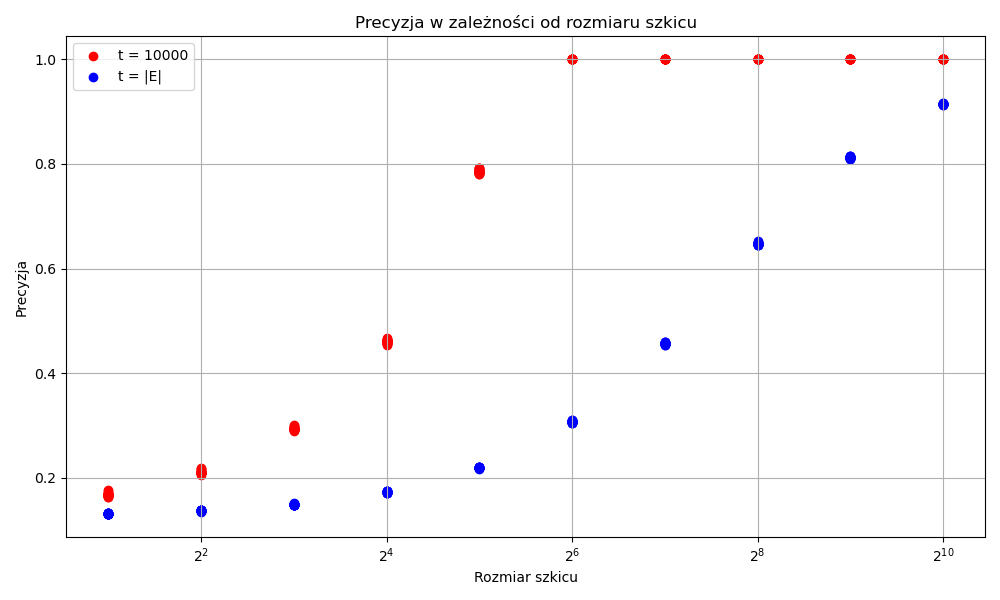
\includegraphics[width=16cm]{img/precision_m.png}
        \centering
        \label{fig:precision_m}
        \caption[Precyzja rekonstrukcji]{Precyzja rekonstrukcji w zależności od rozmiaru szkicu dla algorytmu EdgeSketch.}
    \end{figure}
    
    \subsection{Wnioski}
    Zgodnie z intuicją, zwiększenie rozmiaru szkicu ma korzystny wpływ na uzyskiwaną precyzję. Algorytm EdgeSketch jest szczególnie widoczne w przypadku dużych wartości $t$. Warto jednak zaznaczyć, że im większy szkic, tym dalsze jego zwiększanie ma mniejszy wpływ na precyzję. Co ciekawe, dla małych $t$, EdgeSketch jest w stanie uzyskać wysoką precyzję nawet przy małym rozmiarze szkicu. Przykładowo, dla $t = 10000$, szkic o rozmiarze $64$ jest wystarczający, aby w każdym z badanych przypadków uzyskać precyzję $1$, a w dla zbioru dblp, wystarczający jest nawet szkic o $8$ elementach. W przypadku algorytmu NodeSketch, zyski występują, ale są niewielkie w porównaniu do EdgeSketcha. Warto zaznaczyć, że większy rozmiar szkicu implikuje większą liczbę wykonywanych operacji oraz większe zapotrzebowanie na pamięć, dlatego w praktycznych zastosowaniach konieczne może być znaleznienie kompromisu pomiędzy jakością uzyskiwanych wyników a kosztem obliczeniowym.

\section{Dobór parametru alpha}

    Kolejnym parametrem, mającym znaczenie dla obu algorytmów jest $\alpha$. Jego wartość decyduje, jak szybko maleje wpływ kolejnych, coraz bardziej odległych sąsiadów na generowane szkice, lub, w przypadku EdgeSketcha, obliczane podobieństwa Jaccarda. Grafy wykorzystane w eksperymencie zostały wygenerowane w modelu Erdosa-Renyiego i miały $5000$ wierzchołków. Badano różne wartości $\alpha \in \{0, 0.15, 0.3, 0.45\}$, przy czym $\alpha = 0$ oznacza, że sąsiedztwa wyższych rzędów nie były brane pod uwagę. Rozmiar szkicu $m$ ustalono na $10$, a parametr $k$ na $4$. Rezultaty przedstawiono w tabeli \ref{tab:alpha}.

    \begin{table}[!ht]
        \small
        \centering
        \begin{tabular}{|l|l|l|l|l|l|l|l|l|l|}
        \hline
            & & \multicolumn{4}{c|}{NodeSketch} & \multicolumn{4}{c|}{EdgeSketch} \\ \cline{1-10}
            \textbf{p} & \textbf{$\alpha$} & \textbf{t = 100} & \textbf{t = 1000} & \textbf{t = 10000} & \textbf{t = |E|} & \textbf{t = 100} & \textbf{t = 1000} & \textbf{t = 10000} & \textbf{t = |E|} \\ \hline\hline
        \multirow{4}{*}{0.0005} & 0 & 0.97 & 0.826 & 0.3424 & 0.5415 & 1 & 1 & 0.4462 & 0.7057 \\ \cline{2-10}
            & 0.15 & 0.9 & 0.798 & 0.2917 & 0.4613 & 1 & 1 & 0.4678 & 0.7398 \\ \cline{2-10}
            & 0.3 & 0.95 & 0.782 & 0.2863 & 0.4528 & 1 & 1 & 0.4363 & 0.69 \\ \cline{2-10}
            & 0.45 & 0.9 & 0.788 & 0.2743 & 0.4338 & 1 & 0.785 & 0.3954 & 0.6253 \\ \hline\hline
        \multirow{4}{*}{0.001}    & 0 & 0.91 & 0.69 & 0.4114 & 0.3773 & 1 & 1 & 0.6996 & 0.5548 \\ \cline{2-10}
            & 0.15 & 0.15 & 0.056 & 0.0168 & 0.0146 & 1 & 1 & 0.7469 & 0.6264\\ \cline{2-10}
            & 0.3 & 0.16 & 0.047 & 0.0185 & 0.0164 & 1 & 0.996 & 0.7014 & 0.6161 \\ \cline{2-10}
            & 0.45 & 0.19 & 0.069 & 0.0198 & 0.0173 & 0.97 & 0.939 & 0.6041 & 0.5373 \\ \hline\hline
        \multirow{4}{*}{0.005}    & 0 & 0.38 & 0.258 & 0.144 & 0.0972 & 1 & 1 & 1 & 0.1814 \\ \cline{2-10}
            & 0.15 & 0 & 0.007 & 0.0049 & 0.0053 & 1 & 1 & 0.9276 & 0.1871 \\ \cline{2-10}
            & 0.3 & 0 & 0.004 & 0.0042 & 0.005 & 1 & 0.932 & 0.3196 & 0.1062 \\ \cline{2-10}
            & 0.45 & 0 & 0.006 & 0.0044 & 0.0052 & 0.95 & 0.381 & 0.1227 & 0.0559 \\ \hline\hline
        \multirow{4}{*}{0.01}    & 0 & 0.15 & 0.185 & 0.1091 & 0.0563 & 1 & 1 & 1 & 0.1011 \\ \cline{2-10}
            & 0.15 & 0.01 & 0.011 & 0.0101 & 0.0094 & 1 & 1 & 0.9231 & 0.1022 \\ \cline{2-10}
            & 0.3 & 0.01 & 0.009 & 0.0095 & 0.0095 & 1 & 1 & 0.3234 & 0.0647 \\ \cline{2-10}
            & 0.45 & 0.01 & 0.009 & 0.0094 & 0.0095 & 1 & 0.63 & 0.1928 & 0.0428 \\ \hline
        \end{tabular}
        \label{tab:alpha}
        \caption{Wyniki dla różnych wartości parametru $\alpha$}
    \end{table}

    \subsection{Wnioski}
    Odpowiedni dobór paramtru rozkładu wykładniczego zależy od konkretnego grafu. W badanym modelu dla algorytmu NodeSketch najlepsze wyniki uzyskano ignorując sąsiedztwa wyższych rzędów. Inaczej było w przypadku EdgeSketcha, gdzie niewielkie wartości parametru, zwłaszcza $\alpha = 0.15$ lub $\alpha = 0.3$ wływały korzystnie na uzyskiwane wyniki. Pogarszały się one jednak przy wyborze większych współczynników. Większa $\alpha$ pozwala na ujęcie większej ilości informacji o dalszym sąsiedztwie, ale może również przykrywać informacje o najbliższych sąsiedach wierzchołka, co później zaburza proces rekonstrukcji krawędzi. W większości przypadków wybór małych wartości $\alpha$ wydaje się więc najskuteczniejszą strategią dla algorytmu NodeSketch. 

\section{Liczba operacji w zależności od liczby krawędzi w grafie}
    Teoretyczna złożoność obliczeniowa algorytmów NodeSketch i EdgeSketch została skomentowana w rozdziale \ref{sec:complexity}. Analiza ta obejmowała wszystkie kroki wykonywane w trakcie działania algorytmów. Jednak w praktyce, pewne operacje mogą mieć o wiele istotniejszy wpływ na ostateczny czas działania niż inne. W szczególności, obliczenie wartości funckji haszujące, choć odbywa się w czasie $O(1)$, to przy dużej liczbie wywołań ma znaczący wpływ na efektywność algorytmu. W poniższym eksperymencie zbadano średnią liczbę obliczonych wartości funkcji haszujących w zależności od liczby krawędzi w grafie. W tym celu wygenerowano grafy w stochastycznym modelu blokowym o różnych rozmiarach, od $200$ do $8000$ wierzchołków. Wszystkie z nich miały $4$ bloki, a prawdopodobieństwa krawędzi wewnątrz bloku i pomiędzy blokami wynosiły odpowiednio $0.5$ i $0.001$. Podobnie jak w innych eksperymentach, rozmiar szkicu $m$ wynosił $10$ i przyjęto $\alpha = 0.3$. Wyniki przedstawiono na wykresie \ref{fig:calculated_hashes_vs_edges_all}. Dodatkowo, wykres \ref{fig:calculated_hashes_vs_edges_relative} przedstawia te same wyniki, ale znormalizowane względem liczby krawędzi w grafie. Warto zaznaczyć, że w implementacji algorytmu NodeSketch zastosowano podobną optymalizację jak w algorytmie EdgeSketch, polegającą na obliczanniu wartośći funkcji haszującej tylko dla niezerowych elementów w macierzy $SLA$. 

\begin{figure}[!ht]
    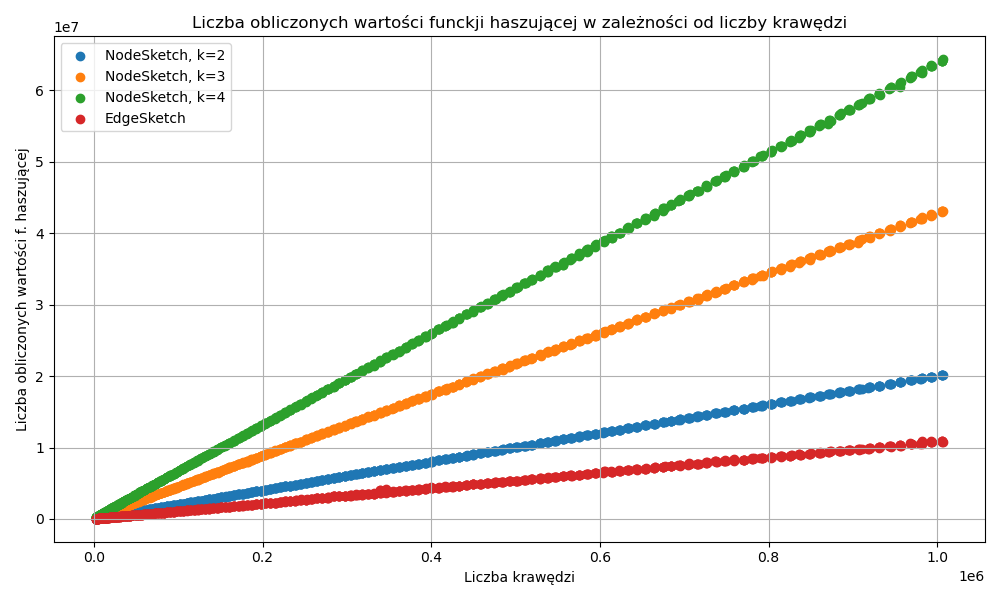
\includegraphics[width=16cm]{img/calculated_hashes_vs_edges_all.png}
    \centering
    \label{fig:calculated_hashes_vs_edges_all}
    \caption[Liczba operacji]{Liczba obliczonych wartości funkcji haszującej w zależności od liczby krawędzi w grafie}
\end{figure}

\begin{figure}[!ht]
    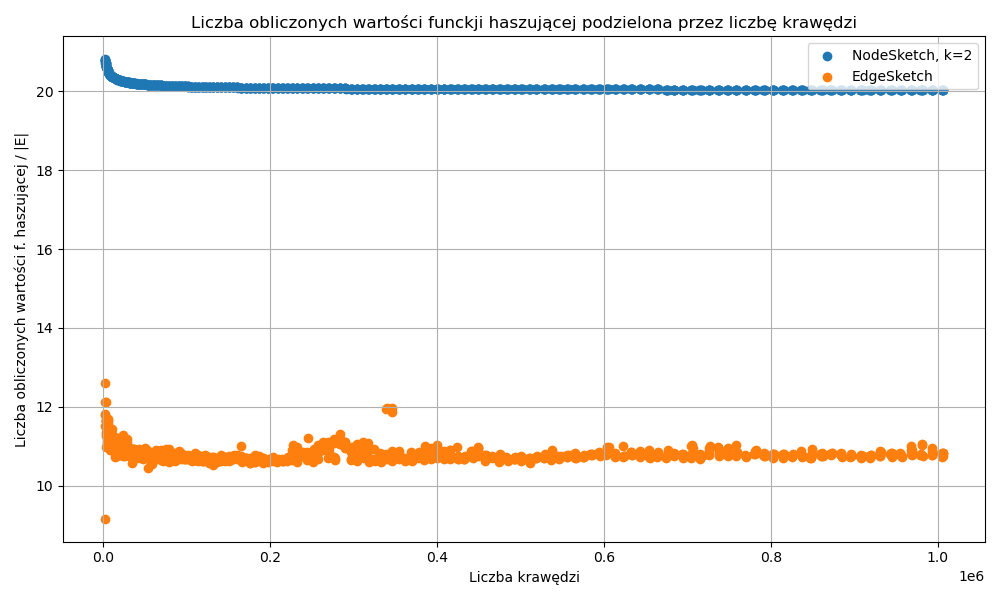
\includegraphics[width=16cm]{img/calculated_hashes_vs_edges_relative.png}
    \centering
    \label{fig:calculated_hashes_vs_edges_relative}
    \caption[Liczba operacji znormalizowana]{Liczba obliczonych wartości funkcji haszującej znormalizowana względem liczby krawędzi w grafie}
\end{figure}

\subsection{Wnioski}
W przypadku obu algorytmów, liczba wywołań funkcji haszującej rośnie liniowo wraz z liczbą krawędzi w grafie. Jest to spodziewany wynik, ponieważ każda krawędź może być wykorzystywana tylko przy generowaniu zanurzeń dla dwóch wierzchołków, które ją wyznaczają. Jest to także zgodne z teoretyczną złożonością obliczeniową algorytmu EdgeSketch. Zauwazyżmy, że procedura FastExpSketch jest wywoływana $|V|$ razy, a średnia liczba przekazywanych do niej elementów to iloraz liczby krawędzi i liczby wierzchołków, a więc gęstość grafu 
\[
    \rho = \frac{|E|}{|V|},
\]
która w rozważanym modelu jest stała. Ostatecznie otrzymujemy więc:
\[
    O(|V| \frac{|E|}{|V|} \ln(\rho)) = O(|E| \ln(\rho)) = O(|E|)
\]

Wraz ze wzrostem parametru $k$, NodeSketch wykonuje więcej operacji ze względu na rekurencyjną procedurę szkicowania. Oczywiście EdgeSketch generuje zanurzenia tylko raz, co daje mu porzewagę przy rozważaniu wyższych stopni sąsiedztwa. Jednak nawet dla $k = 2$, EdgeSketch wykonuje wyraźnie mniej wywołań funckji haszującej niż NodeSketch.

Na drugim wykresie widać ukazującym liczbę wywołań podzieloną przez liczbę krawędzi, widać, że stosunek ten jest rzeczywiście liniowy. Jedynie dla małych grafów odznaczają się nieco większe wartości. Wynika to z faktu, że algorytmy wykorzystują macierz $SLA$, a nie zwykłą macierz sąsiedztwa, a więc biorą pod uwagę sztuczną pętle od wierzchołka do siebie samego, nie ujętą w zaprezentowanej liczbie krawędzi. Dla algorytmu NodeSketch stosunek ten stabilizuję się na ok $20$. Wynika to z faktu, że szkic ma rozmiar $10$, a każdą z krawędzi rozważamy dla dokładnie dwóch wierzchołków. Wykorzystanie procedury FastExpSketch pozwala zredukować tę wartość prawie dwukrotnie, choć jest to okupione większą wariancją.  

\label{sec:performance}
% LITERATURA (zostanie wygenerowana automatycznie)
%UWAGA: bibliotekę referencji należy przygotować samemu. Dobrym do tego narzędziem jest JabRef.
%       JabRef oferuje jednak większą liczbę typów rekordów niż obsługuje BibTeX.
%       Proszę nie deklarować rekordów o typach nieobsługiwanych przez BibTeX.
%       Formatowania wykazu literatury i cytowań odbywać się ma zgodnie z zadeklarowanym stylem.
%       Zalecane są style produkujące numeryczne cytowania (w postaci [1], [2,3]).
%       Takim stylem jest np. plabbrv
\bibliographystyle{plabbrv}
%       Aby zapanować nad odstępami w wykazie literatury można posłużyć się poniższą komendą
\setlength{\bibitemsep}{2pt} % - zacieśnia wykaz
%       Pozycja Literatura pojawia się w spisie treści nieco inaczej niż spisy rysunków, tabel itp.
%       Aby zachować właściwe odstępy należy użyć poniższej komendy
\addtocontents{toc}{\addvspace{2pt}} % ustawiamy odstęp w spisie treści przed pozycją Literatura 
%       Nazwę pliku przygotowanej biblioteki wpisuje się bez rozszerzenia .bib
%       (linia poniżej załaduje rekordy z pliku "dokumentacja.bib")
\bibliography{dokumentacja}
\appendix

\end{document}
